\label{ch:res}
%In the previous chapters, many different methods that can be used to compute PESs numerically are described and in chapter \ref{ch:proced} the method used within this work is described in more detail.
%In this chapter some results are shown and explained.
Since the method developed in this work combines several techniques that have not been used together so far and quantum-mechanical continuum-function are not treated with the infinite elements technique so far, several conceptual questions need to be clarified before computing actual PESs.
In section \ref{ch:BCbench}, infinite elements are compared with Dirichlet BCs and their respective influence on the properties of the wave function is studied. %In section \ref{sec:NumConve} further benchmarking calculations on some numerical parameters are shown.
These calculations are performed using atomic lithium and hydrogen as test system.
Especially the case of hydrogen is of interest here since analytic solutions to compare with are available.
Thereafter, in section \ref{sec:cs}, the energy-dependence of the cross section for the valence transition of lithium as well as several transitions of carbondioxide are studied, comparing several theoretical approaches with experimental data.
Moreover, the PESs of CO$_2$ and benzene as computed with several theoretical approaches are shown.

\section{Comparison of Boundary Conditions}
\label{ch:BCbench}
In section \ref{ch:BC}, several BCs which give rise to different properties for the solution have been briefly overvied.
Detailed studies on absorbing BCs, non-reflecting BCs as well as complex absorbing potentials can be found in literature \cite{babuska,artBC,capComp,absRev,nrBCrev}.
In this work, Dirichlet boundaries and infinite elements are studied in more detail and the properties of the respective results are compared.
Even though the validity of Dirichlet BCs is questionable for unbound problems, they are easy to apply and their physical consequences provide quite straightforward interpretation of the results.
Thus, they provide a good comparison for the study of infinite elements, whose properties are not studied in this context yet.
The infinite elements are the main objective of this work.
Since they provide a reasonable description for outgoing particles, they allow for a small simulation region, even if the wavelength is very large.
Moreover, they have the correct asymptotic behaviour and hence are expected to produce a good representation of continuum solutions.
In section \ref{sec:DBCbench}, systematic tests are made, studying the dependence of the eigenenergies as well as the properties of the wave function on the parameters of the numerical grid used.
Thereafter, in section \ref{sec:iBCbench}, further tests with infinite elements show the influence of these boundary conditions on the solution.
%First, in section \ref{sec:DBCbench} several properties of the grids introduced in section \ref{sec:grid} are studied with Dirichlet boundaries which are particularly easy to set up and understand in their physical consequences provide straightforward interpretation of the results.
%In section \ref{sec:iBCbench}, several properties of the mesh with infinite elements are investigated.
Since it turns out that the solutions obtained with infinite elements are very sensitive to the parameters of mesh and simulation box, this study is performed more extensively.
%For simplicity, the tests shown here are on atomic systems using, unless specified otherwise, an analytic Coulomb potential with charge $1$, corresponding to the ionised hydrogen atom.


\subsection{Dirichlet Boundary Condition}
\label{sec:DBCbench}
Dirichlet boundaries are conceptually the easiest BCs but are known to have a large influence on the solution, especially for continuous functions since they reflect outgoing waves fully.
%\begin{wrapfigure}{l}{0.6\textwidth}
%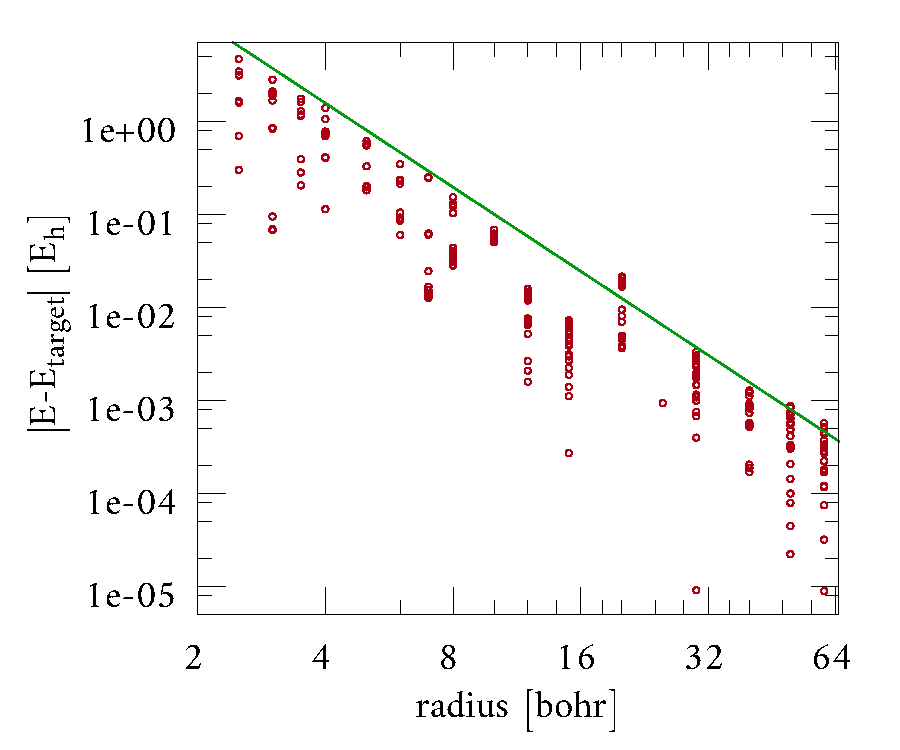
\includegraphics[width=0.6\textwidth]{Figures/BC/DBCenergies}
%\caption{double-logarithmic plot of the error in energy of the energetically closest solutions in dependence on the radius
%of the sphere. The comparison with $\propto \frac{1}{r^3}$ shows the general behaviour of the error.}
%\label{fig:dbcRad}
%\end{wrapfigure}
\begin{figure}
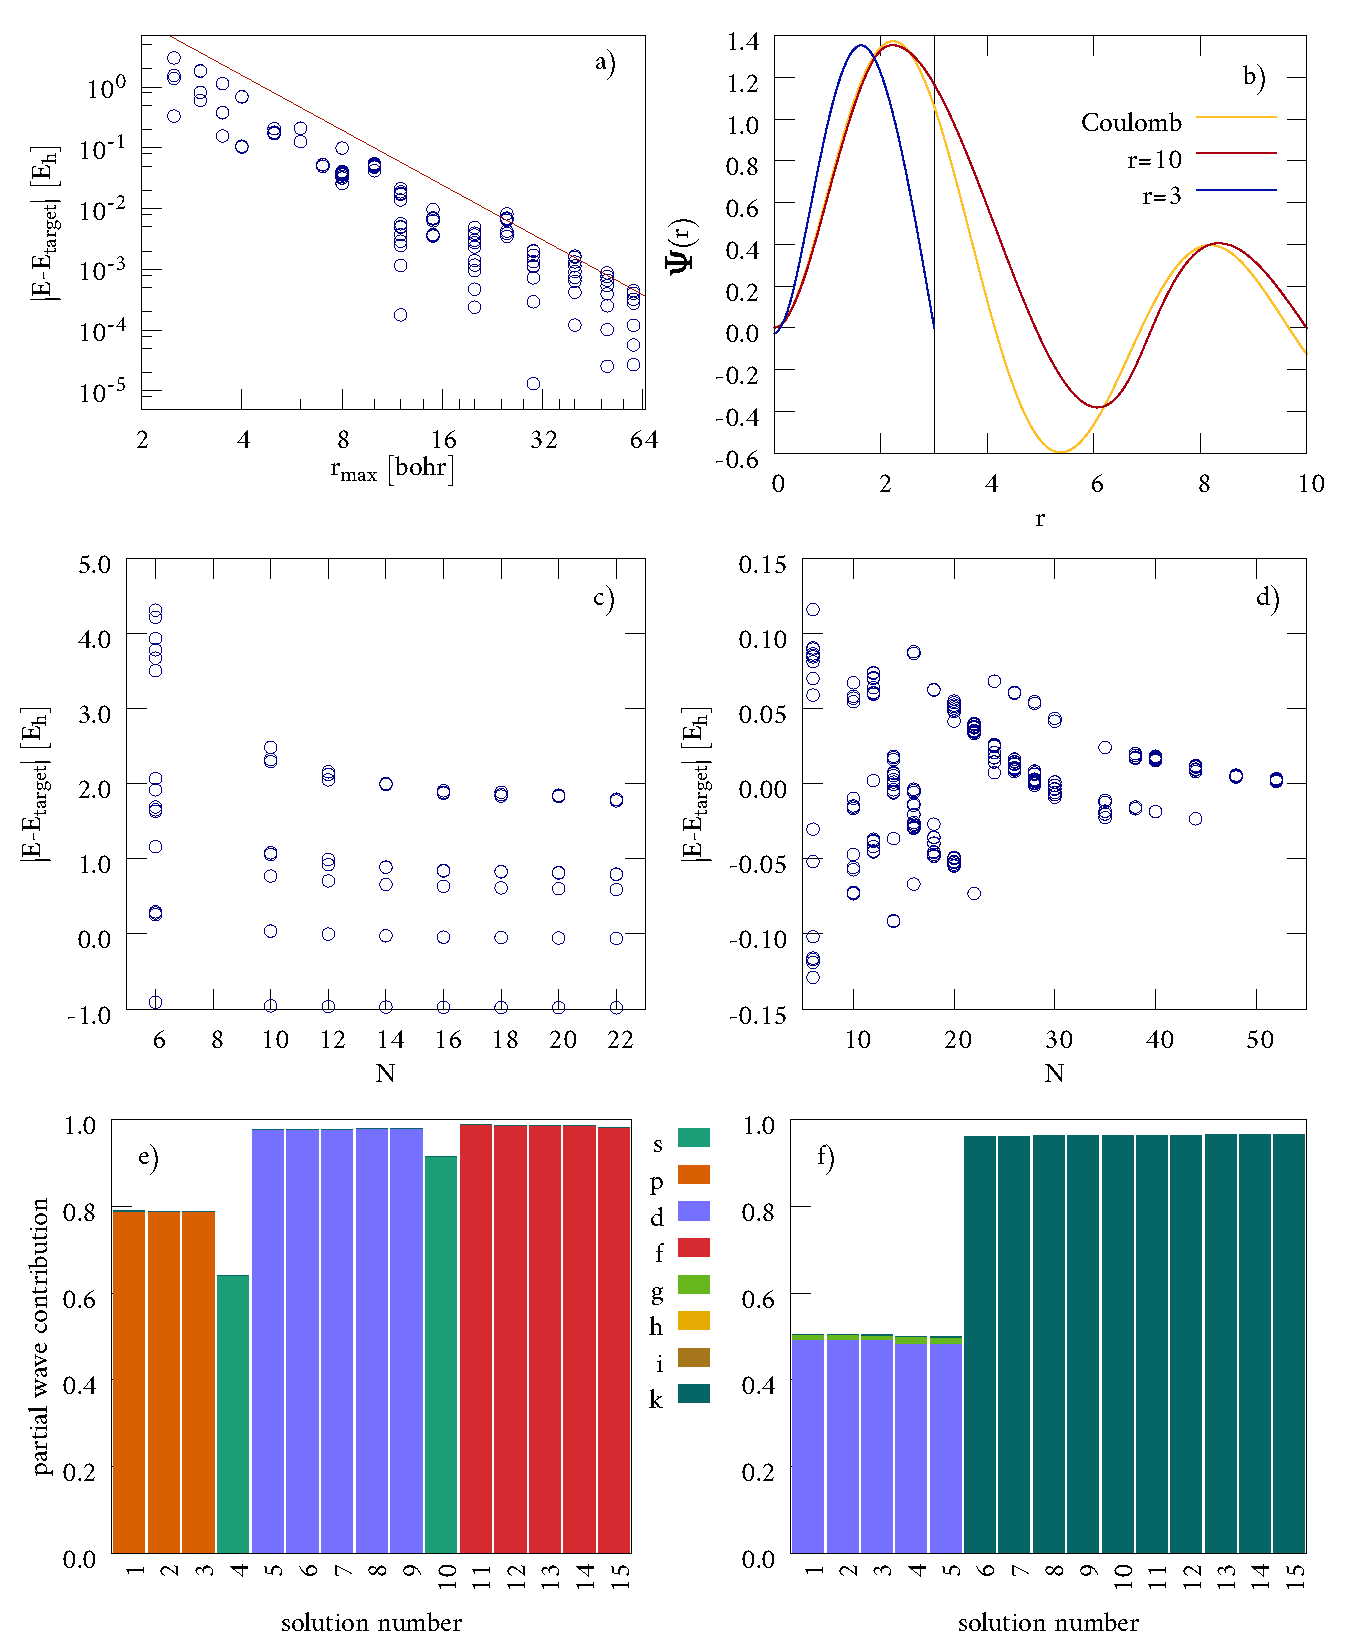
\includegraphics[width=\textwidth]{Figures/BC/DirichletBC}
\caption{Results obtained with Dirichlet BCs using different box sizes:
a) double-logarithmic plot from the deviation in energy for the solutions closest to the target energy $E_\text{target}=0.566\,$Hartree as a function of the radius of the simulation box;
b) real part of $d$-wave functions obtained with different boxes ($r_\text{max}=3\,$bohr and number of spheres $N=18$, blue line and $r_\text{max}=10\,$bohr and $N=38$ spheres, red line); Coulomb wave (yellow line) is also presented for comparison;
c) and d) show the deviation in energy for box radii of $3\,$ and $10\,$bohr,\ varying the number of spheres (radial grid density, see \eq{eq:tm_map}) in the box;
e) and f) show the partial wave contributions \eq{eq:PartWaveCoeff} having different angular momenta for the the respective solutions with $r_\text{max}=3$ and $N=16$ (left) as well as $r_\text{max}=10$ and $N=38$, respectively.}
\label{fig:dbcRad}
\end{figure}
Moreover, its requirement for the solutions to vanish at the boundaries results in an artificial discretisation of the spectrum similar to that of bound states.
This leads to a banded spectrum, with the energy gap between two states being dependent on the simulation box size.
%Moreover, these boundaries enforce the real and imaginary part of the solution to be identical up to a scaling operations (such as rotations and reflections for spherical systems) which does not hold for continuum waves such as Coulomb waves as can be seen in Figure \ref{fig:RadFun} and plane waves that have a constant phase shift.

%These properties are found in various tests conducted to find reasonable parameters for application to more complex systems.
To understand the general properties of solutions for Dirichlet BC and to formulate requirements to the mesh quality, the method has been first tested on the hydrogen-like system with $\nicefrac{1}{r}$ ESP.
To do so, the radius of the simulation box $r_\text{max}$ and the number of spheres, $N$, see \eq{eq:tm_map} has been varied to get convergent results.
In Figure \ref{fig:dbcRad} a), the deviation in the energy of $15$ solutions is shown for different $r_\text{max}$ (see \eq{eq:tm_map}), the number of spheres is kept constant at $N=20$.
The comparison with the red line that represents a $\nicefrac{\text{const}}{r^3}$ dependence, shows that the error is inverse proportional to the volume of the box which is a well-known result for particles in a box with infinite potential walls. 
The number of spheres is kept constant at $N=20$.
The influence of radial grid density on the energies is shown in the panels c) and d) of Figure \ref{fig:dbcRad} where the number of spheres is varied for two different box-sizes, $r_\text{max}=3$ and $r_\text{max}=10\,$bohr, respectively.
In these figures several branches of solutions can be seen that correspond to different angular momenta.
For smaller radii ($r_\text{max}=3\,$bohr, panel c)), these branches are well-separated but become closer and interfere with each other at larger radii ($r_\text{max}=10\,$bohr, panel d)).
Following the expectations, the energies of the respective branches decay when the number of grid points.
At $N=18$ for $r_\text{max}=3\,$bohr the results converge and do not change much with further increase of $N$.
However, for $r_\text{max}=10\,$bohr the convergence is much slower and cannot be reached for $N<60$.
In principle, the continuum spectrum should have infinite degeneracy containing FEFs corresponding to arbitrary angular momenta and since larger boxes provide higher density of states it may be considered desirable to take as large simulation boxes as possible.
This in general also agrees with the common logic for quantum mechanical calculations.
However, the density of states is not the only important quantity: The PES intensities beinge the main objective in the present work are calculated using the DO.
Due to the aufbau principle, usually the atomic states with quite low angular momentum are populated.
\textit{E.g.} in molecules and atoms consisting of second period elements one can expect only $s$ and $p$ atomic functionals to be populated in the lowest excited electronic states. 
Thus, one can expect that FEFs only up to $l=2$ could contribute to PES intensities if the dipole selection rules hold.
That is why to reproduce reliable intensities, the computational scheme should favour solutions with low angular momentum.

The panels e) and f) of Figure \ref{fig:dbcRad} show the projections of the solutions to the spherical wave functions with respective kinetic energy and different angular momentum, where the partial wave contribution is defined as
\begin{equation} \label{eq:PartWaveCoeff}
\sum_m|\langle \Psi_\text{n} | \Psi_{\vec{k},l,m}^\text{Sph}\rangle |^2.
\end{equation}
Here $|\Psi_{\vec{k},l,m}^\text{Sph}\rangle$ is the spherical wave \eq{eq:spherWave} with angular momentum $l$ and its projection onto the quantisation axis $m$ and $|\Psi_\text{n}\rangle$ denotes the respective numerically obtained solution.
The comparison is done against the spherical waves and not against Coulomb waves, since confluent hypergeometric functions are difficult to converge for larger $r$ and they are much more computationally demanding.

The testcalculations have shown that for the given energy of the photoelectron of $E=0.566\,$ Hartree the obtained solutions have a well-defined angular momentum only for small boxes where the critical radius is in the order of $r_\text{max}=10\,$bohr.
For larger computational domains, the states are mixed and have large contributions from much higher angular momenta and are very sensitive to different parameters such as the number of spheres $N_i$ and the parameters $s$ and $q$ in  \eqs{eq:tm_map} and (\ref{eq:son_map}) respectively.
Moreover, for example the comparison of the Figures \ref{fig:dbcRad} e) and f) shows that solutions with larger boxes tend to have higher angular momenta which is an important argument in favour of smaller boxes since for most atomic systems angular momenta larger than $4$ are not of interest for practical calculations.
This tendencey can be understood when considering the radial SE \cite{Lifschitz}
\begin{equation}
\frac{\partial^2}{\partial r^2} R(r) + \left(2\left(E-V(r)\right) -\frac{l(l+1)}{r^2}\right) R(r)=0
\end{equation}
where $R(r)$ is the radial solution and $E-V(r)$ is identified as kinetic energy.
Thus, given a particular kinetic energy, the radial oscillations are reduced by a larger angular momentum.
This leads to the interpretation that a particle can `distribute' its kinetic energy between the radial (outgoing) and spherical contributions.
In turn, however, needs a wave with large angular momentum more space and thus these solutions are suppressed in smaller computational domains.

In Figure \ref{fig:dbcRad} b), two solutions with $l=2$ along one axis are shown (the fifth one for $r=3$ and the first one for $r=10$ which are shown in \ref{fig:dbcRad} e) and f) as well) for two different box-sizes and compared to the Coulomb wave, being the exact solution for the $-\nicefrac{1}{r}$ potential.
One can see that al both box sizes the radial structure of the wave function can not be reproduced with Dirichlet BC completely, even though the agreement at $r_\text{max}=10\,$bohr is already reasonable.
However, the analytic solution has a node very close to the boundary of the box and thus the agreement will get worse if the maximum radius becomes larger.
This fact is reflected in the energetic difference as well which is in the mE$_\text{h}$-range for the case of $r_\text{max}=10$ whereas the deviation for the smaller box is almost $1\,$Hartree and thus almost twice as high as the target value.
Except for lucky cases where the box-size matches a node of a particular analytic solution, an acceptable deviation in energy of about $10^{-3}\,$Hartree is reached only for box radii of $30\,$bohr or more.
Such simulation setups lead, however, to solutions with very large angular momentum.
Finally, it should be noted that the occurence of high angular momentum solutions is not a problem on its own and should be typical for solutions close to reality.
However, test calculations show that they come out in an unordered way.
Thus, applying some subspace solvers \textit{e.g.} Krylov one, does not guarantee that solutions with low angular momentum will fall in the considered subspace.
This fact does not represent a problem when only energies are accounted for, however, is crucial for PES intensities.

%\subsection{Complex Absorbing Potential}
%Using a CAP as described in section \ref{ch:cap}, two additional degrees of freedom comared to the Dirichlet BCs arise: the strength $\eta$ of the artificial potential (\ref{eq:cap}) and the offset $r_0$ where it starts, the latter has the only restriction to be larger than the radius of the DO.
%In section \ref{ch:cap} it was suggested to chose the parameters such that the respective derivatives of the energy vanish \cite{CAPccEOM,CAPfreshlook}.
%This procedure is, however, only valid if one solution should be taken into account and thus is not directly applicable here.
%Interpreting the real part of the eigenvalues of the eigenproblem (\ref{eq:SEmat}) as the energy of the respective state, the influence of the CAP on the density of states varies strongly when changing other parameters.

\subsection{Infinite Elements}
\label{sec:iBCbench}
The method making use of infinite elements has more different parameters which can be crucial for the stability of the solution than the Dirichlet BC.
Investigations of these dependences is the subject of the present section.
As described earlier, using the infinite element approach, the SE becomes a quadratic eigenvalue problem due to the oscillating contributions in the basis functions \eq{eq:infAnsatz}.
To reduce the computational costs, in this work the frequency of these oscillations is fixed to correspond to a target energy $k=\sqrt{2E_\text{target}}$.
With this the Hamiltonian depends on the target energy and the solutions obtained are with increasing energetical deviation, less consistent.
However, the obtained solutions with a reasonable error in energy are FEF that are adapted to the real ESP that is large in the finite region and show a consistent asymptotic behaviour.
%In the first part of this section, several of the testcalculations shown above for Dirichlet BCs are 

\begin{figure}%{R}{0.5\textwidth}
\begin{subfigure}{0.53\textwidth}
   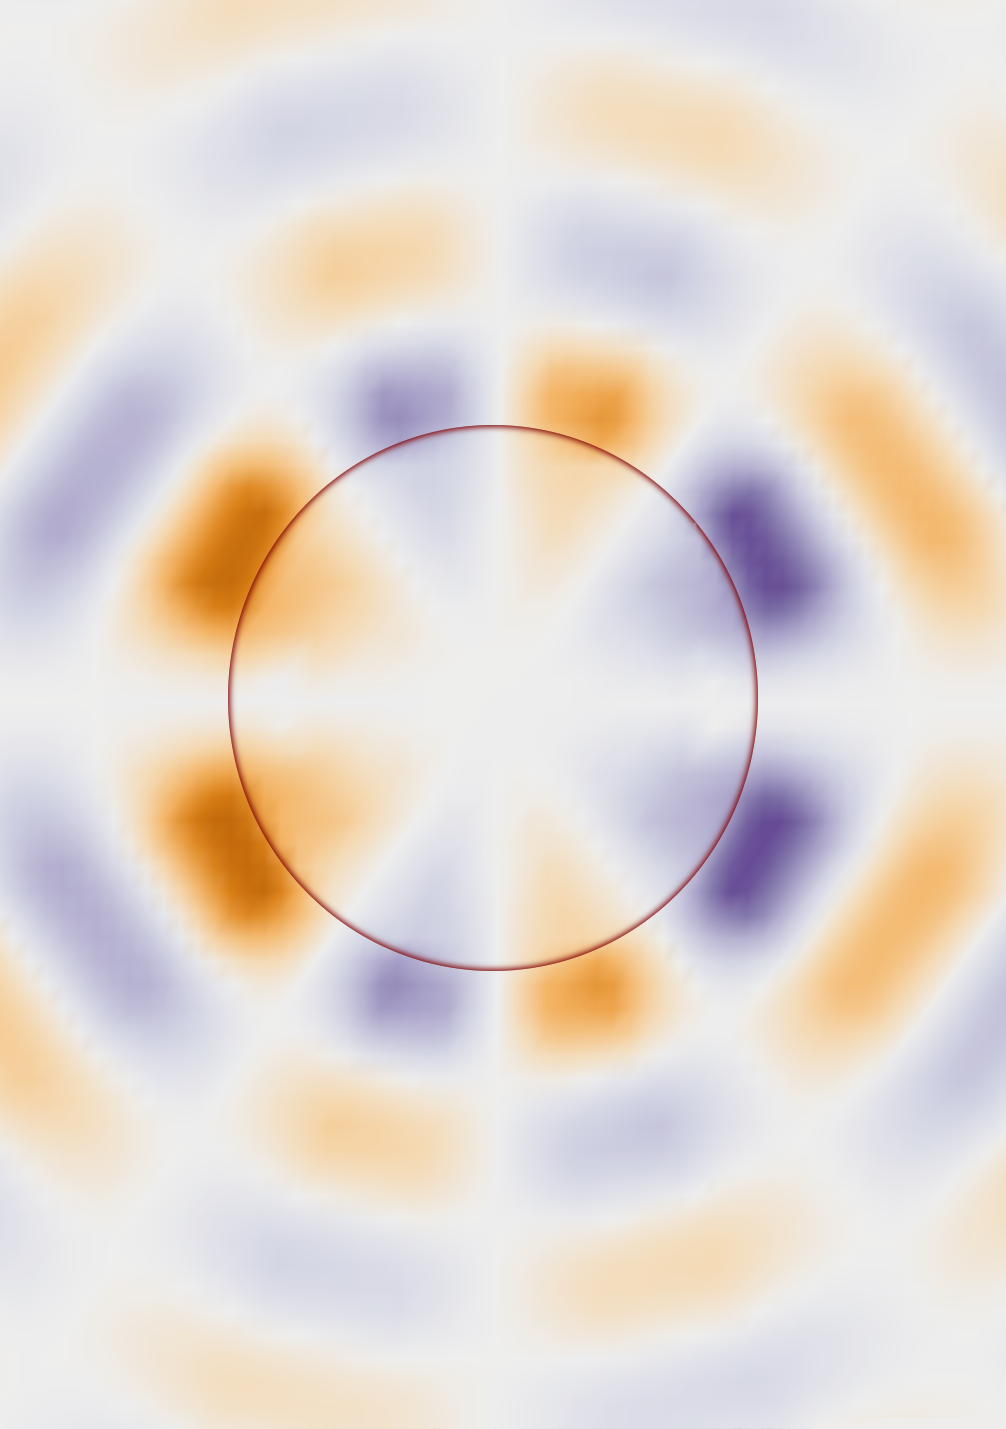
\includegraphics[width=\textwidth]{Figures/BC/plane_fin}
   \caption{2D-cut through a FEF obtained with infinite elements using a spherical finite element region indicated by the red circle with a radius of $r=6\,$bohr and $N=11$ spheres for a target energy of $E_\text{target}=2.12\,$Hartree.}
   \label{fig:cutInfa}
\end{subfigure}
\begin{subfigure}{0.47\textwidth}
   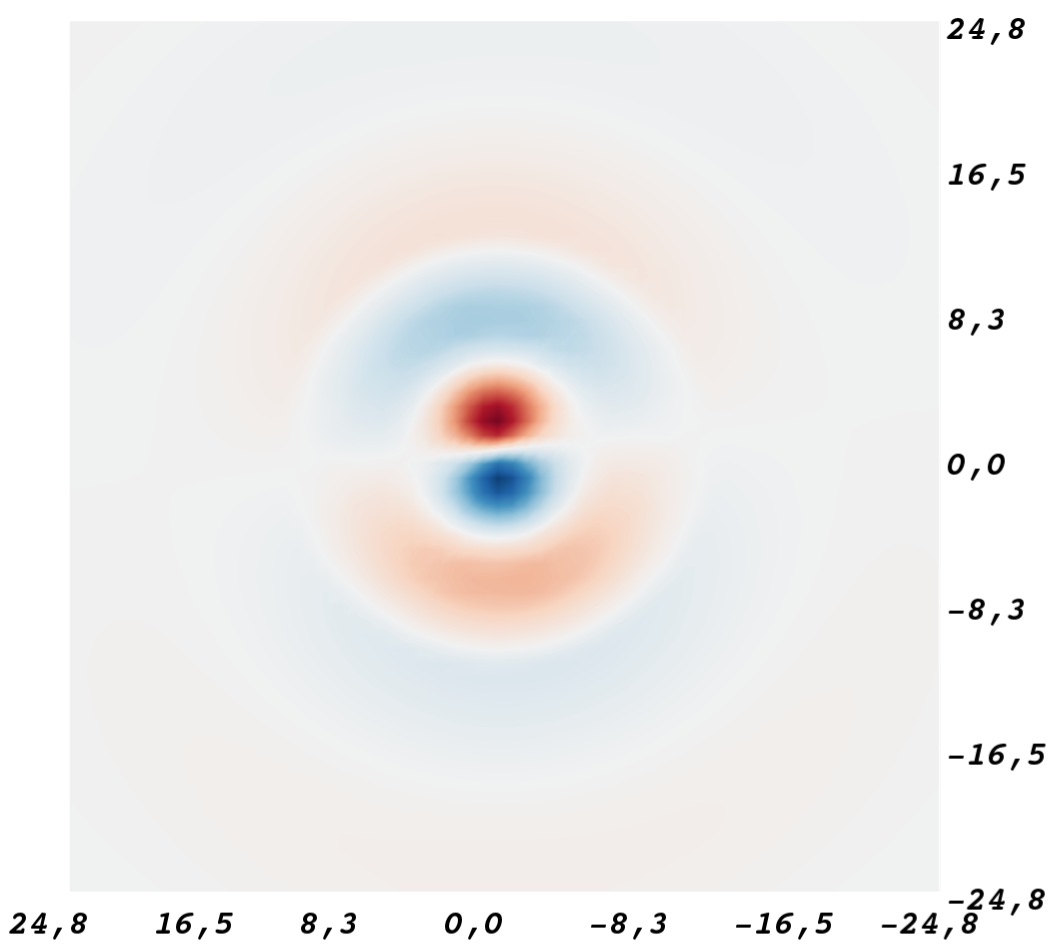
\includegraphics[width=\textwidth]{Figures/RBF/p_wave}
   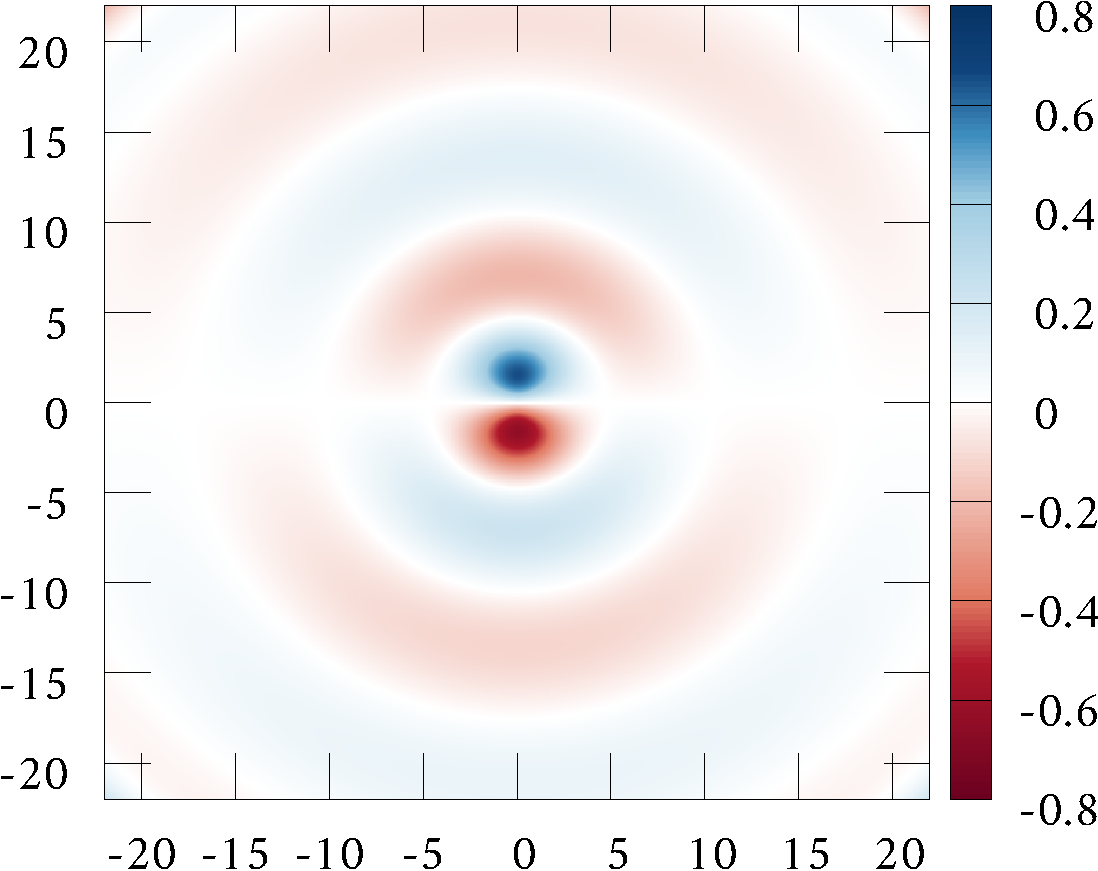
\includegraphics[width=\textwidth]{Figures/RBF/P-Wave}
   \caption{2D-cut through a FEF obtained with angular momentum $l=1$ (upper panel) and the respective analytic Coulomb wave (lower panel) for comparison.
   Box-parameters of the numerical setup: $r_\text{max}=12.39$, $N=18$, radial scheme: tm \eq{eq:tm_map}, $s=2.5$, $q=1.2$, $E_\text{target}=0.133\,$Hartree.}
   \label{fig:cutInfb}
\end{subfigure}
%\caption{Solutions obtained with different parameters }
\label{fig:cutInf}
\end{figure}
In Figure \ref{fig:cutInf}, the 2D-cut of typical solutions obtained with infinite elements for the hydrogen atom are shown.
The red circle in Figure \ref{fig:cutInfb} indicates the region of finite elements.
These graphs illustrate the the asymtotic behaviour of the regular oscillations of an outgoing wave with correct wavelength.
Moreover, the comparison of the numerically obtained results (upper panel in Figure \ref{fig:cutInfb}) with the respective Coulomb wave (lower panel of Figure \ref{fig:cutInfb}) shows a good agreement.
However, the angular momentum of the solutions in Figure \ref{fig:cutInfa} and \ref{fig:cutInfb} differs considerably and seems to depend strongly on the parameters of the numerical setup.
Thus, a detailed study of this setup as presented in the following chapters is of primary importance to be able to control the main properties of the solution.

%\subsubsection{Formulation of Infinite Elements}
\subsubsection{Comparison of Formulations}
\label{ch:bmFormul}
Before taking a closer look at the convergence of different parameters, first the formulation of infinite elements to be used later is investigated.
To avoid the appearance of infinite integrals and respective surface integrations in the integration of matrix elements as they appear in the Burnett formulation, an additional damping-term $D(r)=\nicefrac{1}{r^{2p}}$ with arbitrary $p>0$ can be introduced.
In the standard Astley-Leis formulation, this term is applied to the test function space with $p=1$, leading to a non-hermitian problem.
It is observed, however, that this damping introduces a suppression of low angular momentum-solutions, even though the solution space remains unchanged.
Since especially the low angular momenta are crucial in this work and to avoid the appearance of complex energies, here the influence of the power $p$ in the damping-term is studied and the symmetrised and non-symmetrised formulations are compared.
%Moreover, to study the influence of the damping function in the Astley-Leis formulation (\ref{eq:ALelem}) in more detail, also a test function space similar to eq. (\ref{eq:ALelem}) but using the squared damping function $D(r)^2$ instead of $D(r)$.

The 50 solutions whose energy is closest to the target value of $0.5675\,$E$_\text{h}$ obtained with the original Astley-Leis formulations with the damping function taken to the powers $p=1$ and $p=2$ as well as the symmetrised formulation (\ref{eq:ALsymm}) suggested in this thesis with powers $p<0.5$ are shown in Figure \ref{fig:IFEMform_spect}.
%For the unsymmetric formulations only the real part is shown which is assigned to the physical energy of the respective state.
For the solutions obtained with the unsymmetric formulation, only the real part is presented in Figure \ref{fig:IFEMform_spect} which is assigned to the physical energy of the respective state.
The eigenenergy of a continuum state determines the frequency of its oscillations if it is a real number.
Inserting a complex number in the oscillating function, its imaginary part leads to a damping of the solution and, using a time-dependent description, to a decaying norm of the wave-function.
\begin{figure}[h]
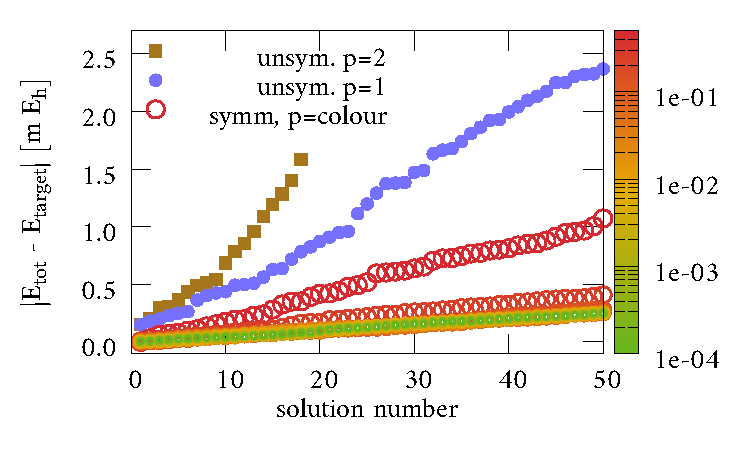
\includegraphics[width=\textwidth]{Figures/IFem_form_spectra}
\caption{The first 50 eigenvalues obtained with the original Astley-Leis formulation (imaginary part not shown) and with the symmetrised form \eq{eq:ALsymm}.
The colorbar denotes the power $p$ of the damping factor $D(r)$ for the symmetric formulation.}
\label{fig:IFEMform_spect}
\end{figure}
Due to this behaviour, complex eigenvalues are interpreted as the energy and lifetime of the respective state.
However, the damping term $D(r)$ that introduces the imaginary part of the eigenvalue is artificial in the case of infinite elements, this lifetime has no physical meaning 
The results presented in Figure \ref{fig:IFEMform_spect} show clearly that the obtained density of states decreases with the power $p$ and converges for $p\approx \frac 18$ for the given parameters (the radial mapping scheme \eq{eq:tm_map} is used with $N=25$, $q=0.5$, $s=2.5$ and $r_\text{max}=7\,$bohr.).
The strong dependence of the obtained spectrum on the power of the damping function indicate that a reasonable asymptotic description is crucial for the properties of the wave function.
Another important conclusion of the , even for small powers $p\approx 10^{-4}$, no numerical instabilities are observed, indicating that the matrix elements are still well-defined.
%The observations made on the convergence-properties using the spectrum in Figure \ref{fig:IFEMform_spect} are supported by the projections of the solutions on spherical waves of which some are shown in Figure \ref{fig:IFEMform_project}.
%
%The dependence of the obtained spectrum of the Hamiltonian on the power of the damping function shows that, at least for FEFs, the asymptotic behaviour is crucial for the properties of the wave function. 
%The dependence converges for $p=1/8$, see also Figure \ref{fig:powerSpect} in supplement.

The fast convergence of the solutions with respect to the power $p$ can be seen also when studying the character of the obtained solutions in terms of the partial wave contribution \eq{eq:PartWaveCoeff}.
In the Figure \ref{fig:IFEMform_project}, the partial wave contribution of $30$ solutions is shown for the original, unsymmetric, Astley-Leis formulation (left panel) and the symmetrised form with different damping powers $p=0.5$ (centre) and $p=10^{-4}$ (right).
The comparison of the solutions obtained with the unsymmetric and the converged ($p=10^{-4}$) symmetric formulation shows that these states have contributions of different angular momenta in a similar ratio.
Especially for low angular momenta, the symmetric formulation seems to be beneficial if the damping is small enough.
\begin{figure}[h]
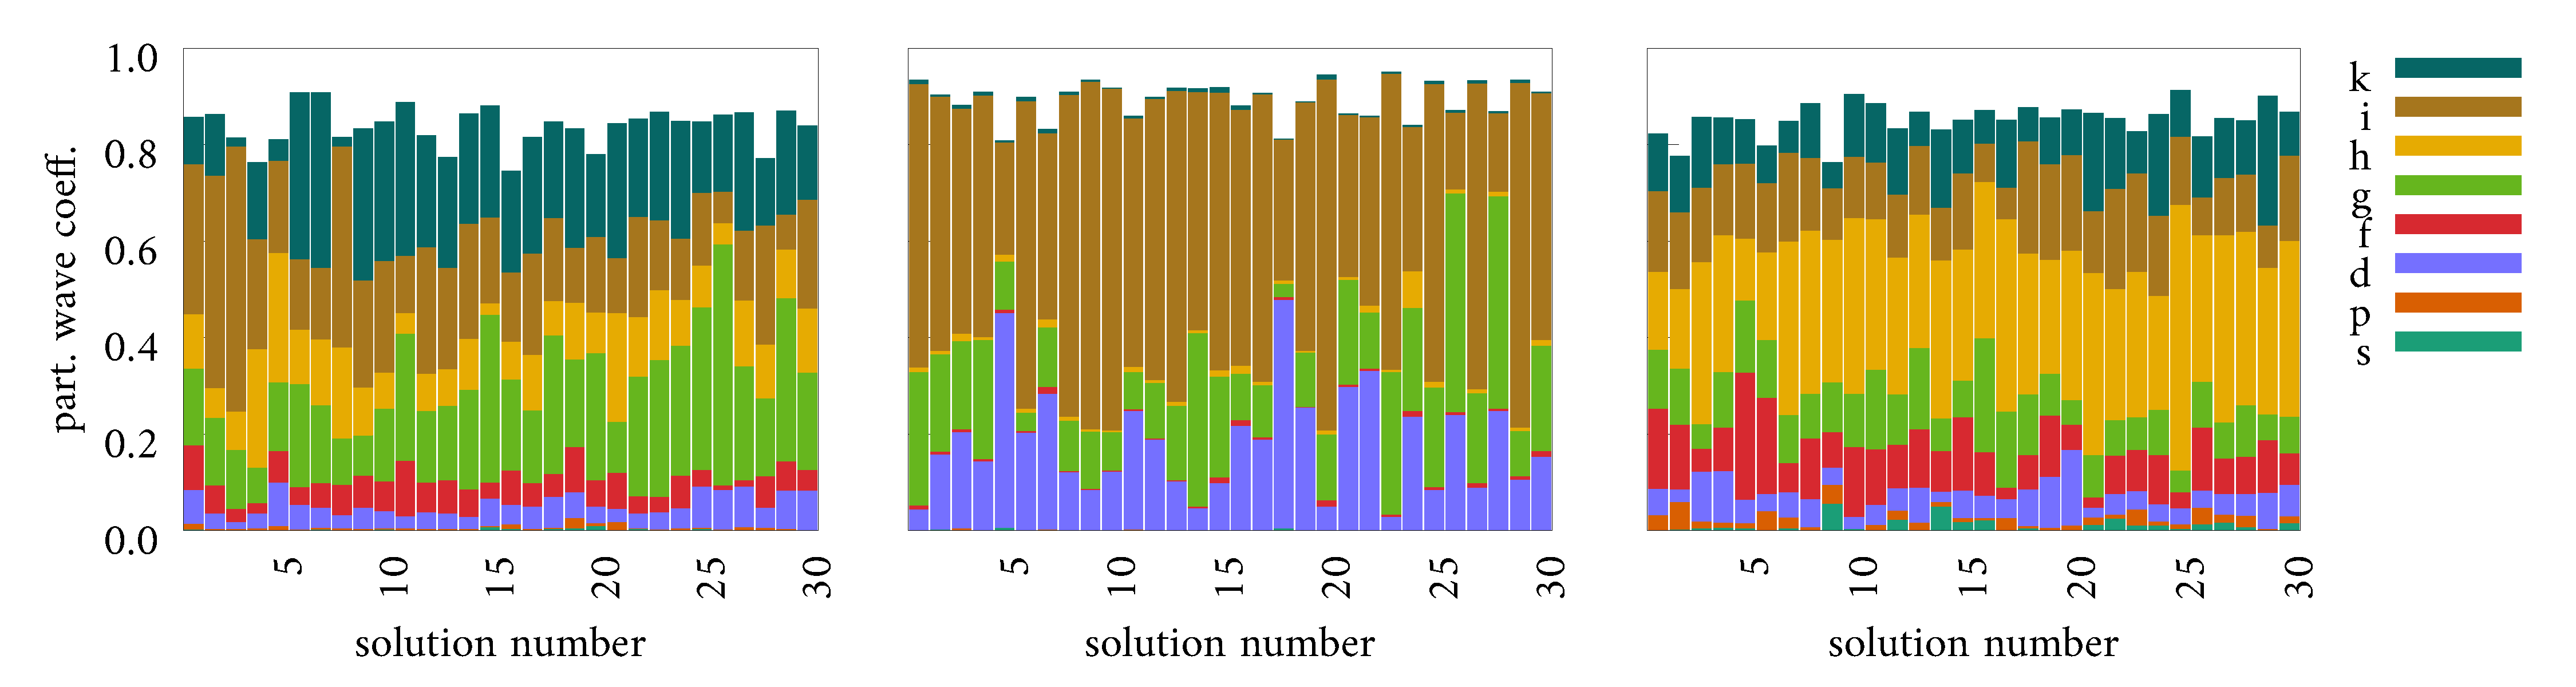
\includegraphics[width=\textwidth]{Figures/Ifem_forms}
\caption{Decomposition of the first $30$ solutions into spherical waves with angular momenta up to $l=7$.
Left: Astley-Leis-formulation ($p=1$), centre: symmetrised form ($p=0.5$) right: symmetrised form ($p=10^{-4}$).}
\label{fig:IFEMform_project}
\end{figure}
However, for larger powers $p$ such as $p=0.5$ as given in the centre panel of Figure \ref{fig:IFEMform_project}, the contributions with angular momentum $l<2$ are completely suppresed.
Hence, even if less contributions of different angular momenta are observed in case of $p=0.5$, the results obtained with this formulation should not be taken into account.
This fact can be understood by considering that the case $p=0.5$ corresponds to an additional factor of $\nicefrac{1}{r}$ in the multipole expansion and thus $s$-waves should be always suppressed in this case.
Chosing the power small enough, however, leads to vanishing influence on the character of the solution.
However, as shown in the Figure \ref{fig:IFEMform_project}, the nature of the states obtained is in all cases strongly mixed in the quantum number $l$ with significant contributions even for $l>7$ which corresponds to the white spaces in Figure \ref{fig:IFEMform_project}.
However, the relative contributions of the angular momenta critically depends on the power $p$, making a reasonable choice of this parameter important.
%Further it is expected that the convergence of $p$ depends on further parameters such as the box-size and kinetic energy of the photoelectron which is, however, not studied here in more detail.
In the rest of this work, the power of the damping function $D(r)$ is chosen to be $p=0.0001$.
This value is by far converged and thus is considered to be reasonable also for other systems.

The mixing od different angular momenta should be, at least in the atomic case, avoidable since the angular momentum operator $\hat{L}$ has the same set of eigensystems as the Hamiltonian.
However, for atomic cases as studied here, the eigenstates should be eigenfunctions of the angular momentum operator $\hat{L}$.
In the analytic case of the hydrogen atom, all angular momenta are degenerate and thus belong to an invariant subspace.
However, for FEFs the discussion of degeneracy is, ambiguous since the solutions are infinitely degenerate at any given energy and thus for any system with radial symmetry a degeneracy of $l$ is present.
It should be noted that this discussion is not true for Dirichlet BC, since these boundaries can be considered as an infinitely high potential well and thus, even in analytic case, the spectrum is discrete and the solutions not degenerate in angular momentum.
%\begin{figure}
%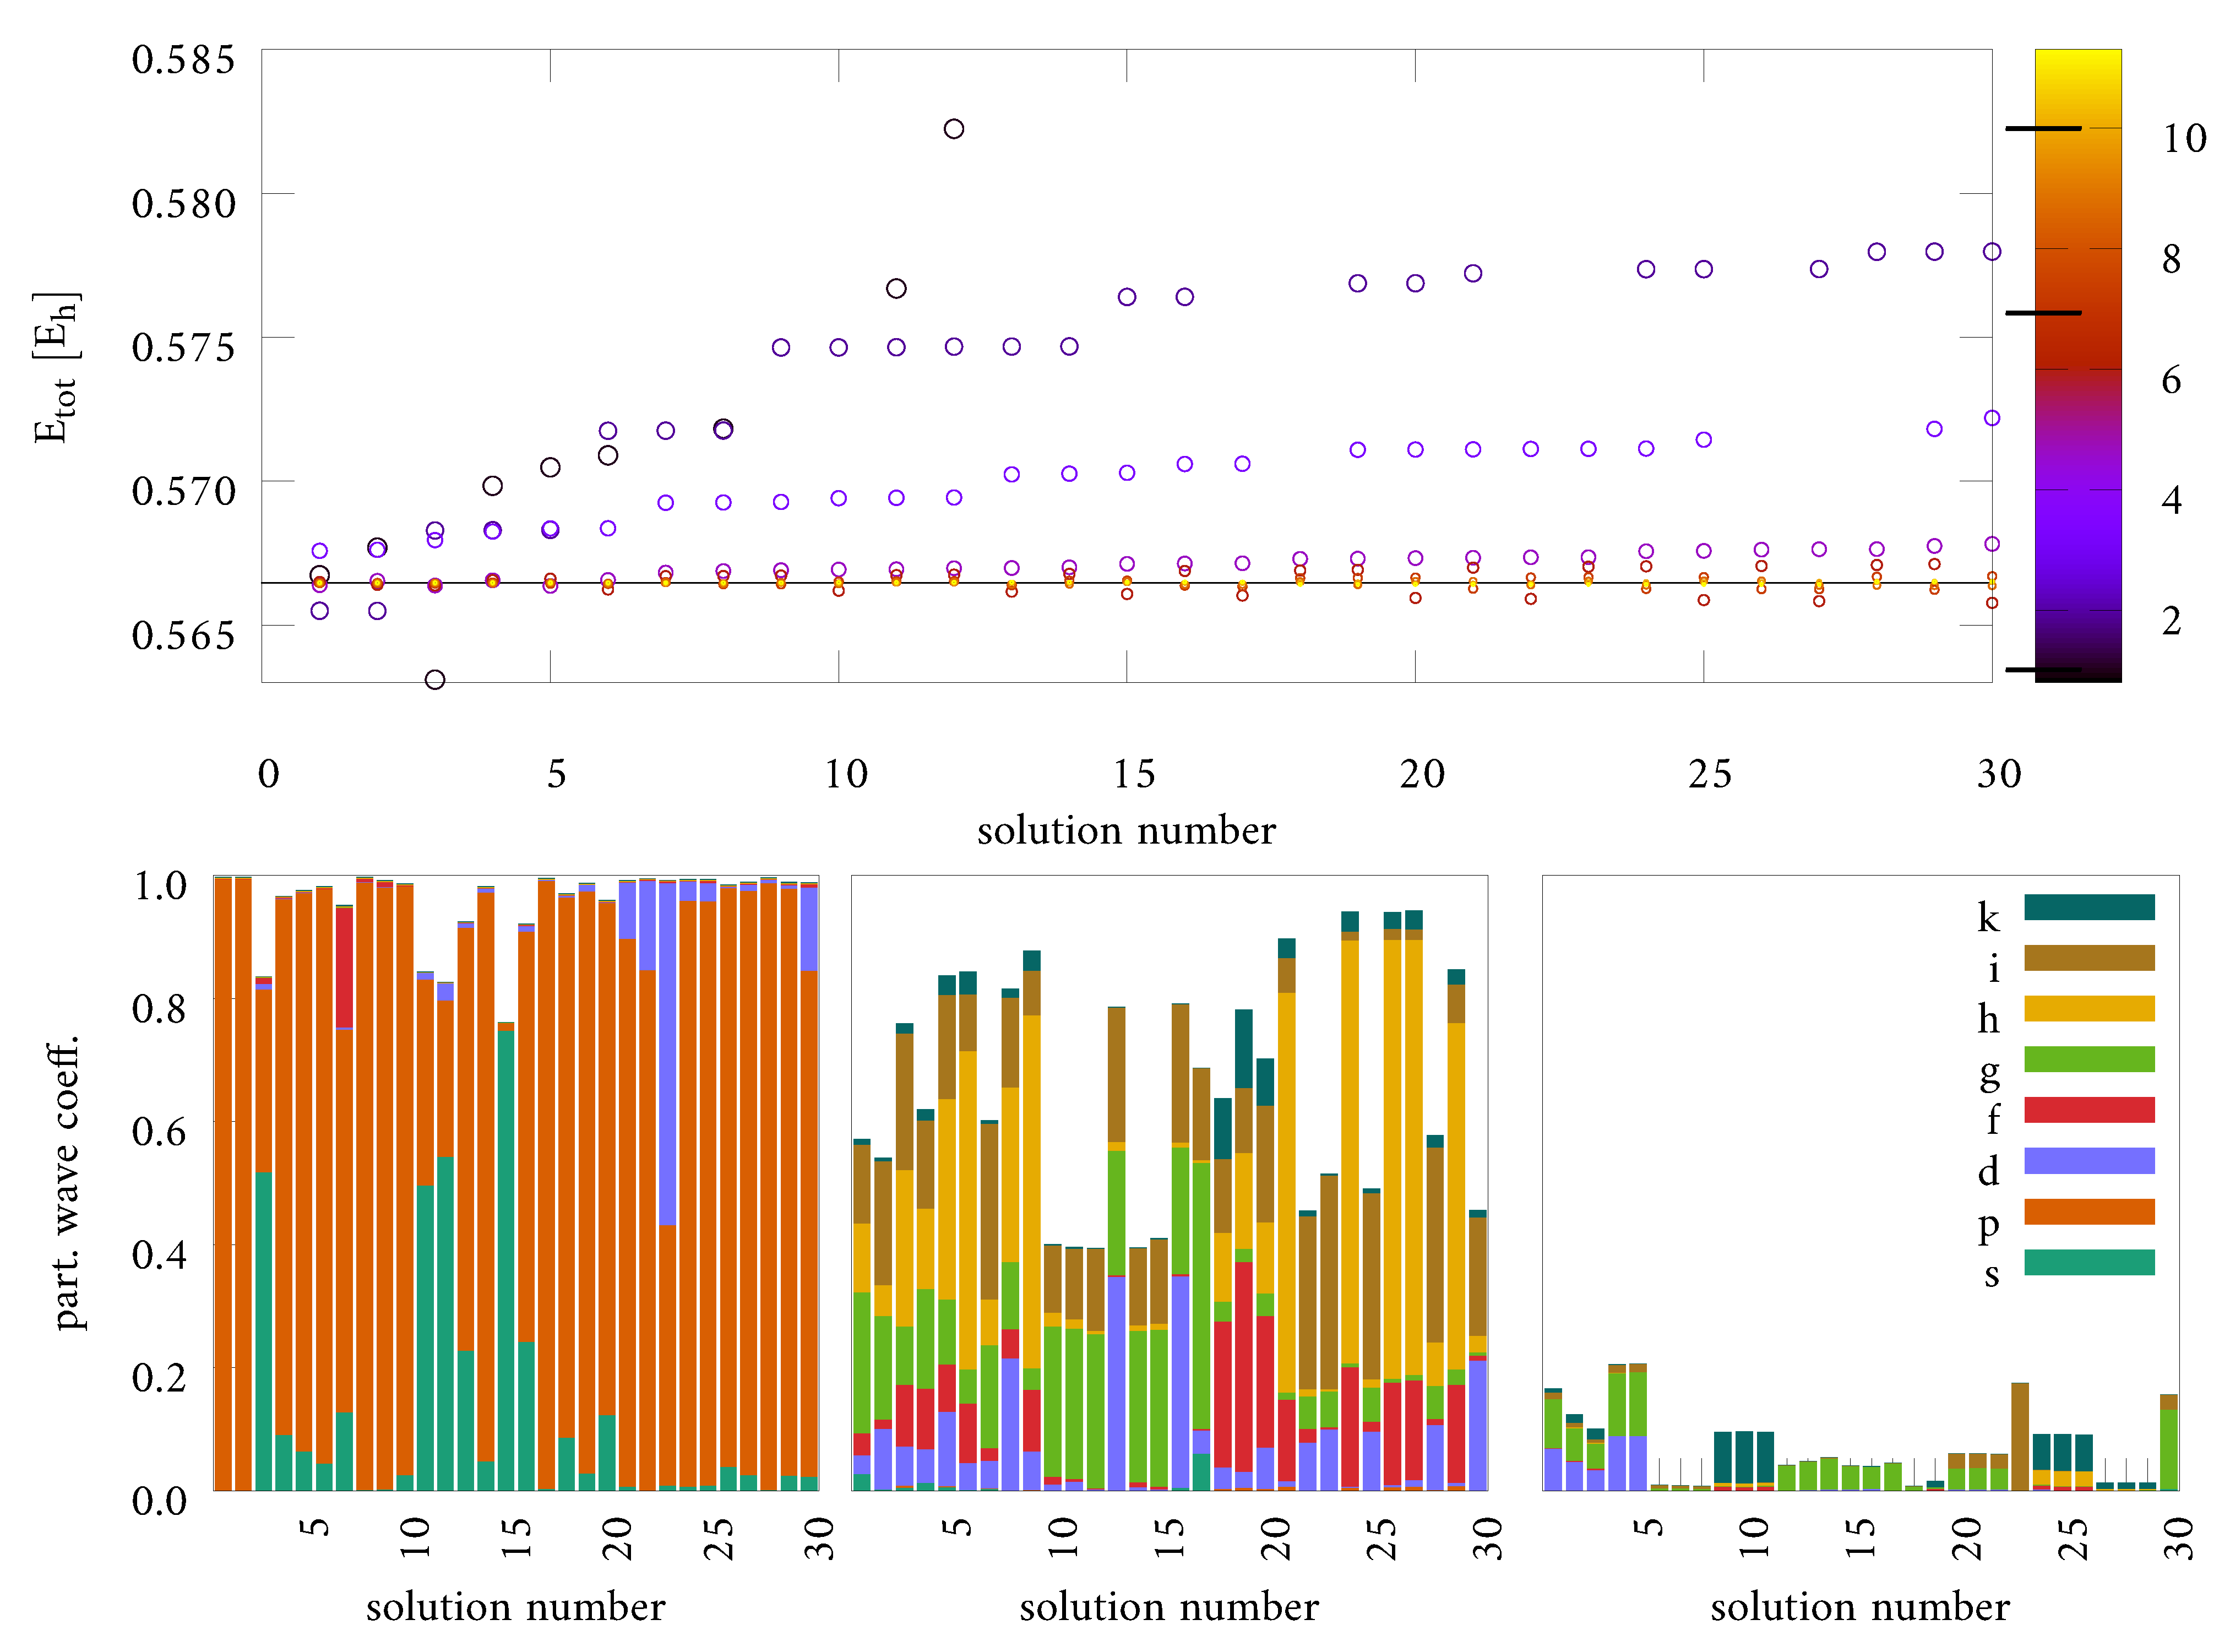
\includegraphics[width=\textwidth]{Figures/RadWave_p0_001.pdf}
%\caption{The eigenenergies for different box sizes (coloured dots in the upper panel) where the box size is denoted by the colour in atomic units.
%The lower panel shows the decomposition of the solutions into spherical waves for three box sizes, marked by a star in the colour bar respectively.}
%\label{fig:RadWaves}
%\end{figure}

Keeping this discussion in mind, the mixing of different angular momenta is caused by the numerical scheme.
The discreteness of the basis in use lifts the infinite degeneracy and, due to numerical irregularities such as the stepwise linear character of the finite element scheme, the high symmetry is disturbed.
It can be shown that the influence of these numerical disturbances on the eigenstates becomes larger, the denser the spectrum is.
Considering the eigensystem $\mat{A}\vec{u}=\lambda\vec{u}$ to be solved, any disturbance can be considered as caused by a matrix $\mat{E}$ that is added to the matrix $\mat{A}$.
Assuming that $\mat{A}$ is a hermitian matrix, the eigenvector $\vec{u}_i$ is changed according to \cite{saad, wilkinson}
\begin{equation}\label{eq:ErrVect}
\delta \vec{u}_i=\sum_{j\neq i} \frac{\vec{u}_j^\dagger\mat{E}\vec{u}_i}{\lambda_i-\lambda_j} \vec{u}_j
\end{equation}
where $\lambda_i$ is the eigenvector corresponding to $\vec{u}_i$.
Accordingly, \eq{eq:ErrVect} represents a direct connection of a dense spectrum and the strong mixing of angular momenta.
%From eq. (\ref{eq:ErrVect}) now the coupling of angular momenta and strong dependence on the parameters for a dense spectrum, \textit{i.e.} small $\lambda_i-\lambda_j$ becomes obvious.

%\subsection{Size of Finite Element Region}
\subsubsection{Radius of the Finite Element Region}
\label{ch:bmSize}
%More important than the subspace used numerically is obviously the size of the sphere used for the FEM description.
Similarly to the Dirichlet BCs discussed in section \ref{sec:DBCbench}, the size of the finite element region has a strong influence on the solution obtained with the infinite BC.
A study of the energies of solutions closest to a target value of $E_\text{target}=0.5664\,$Hartree for different box sizes is presented in Figure \ref{fig:InfBoxc} where, except for the boundary conditions, no parameters are changed with respect to Figure \ref{fig:dbcRad} (a).

Comparison of the respective graphs shows that the error is in general smaller when infinite elements are applied which is an indication for the higher accuracy compared to Dirichlet boundary conditons.
Further, the comparison of the obtained solutions with the $\frac{1}{r^3}$-curve in both figures demonstrates that the dependence is much weaker for infinite elements because the solution is not restricted to decay within the range of the finite box.
\begin{figure}[h]
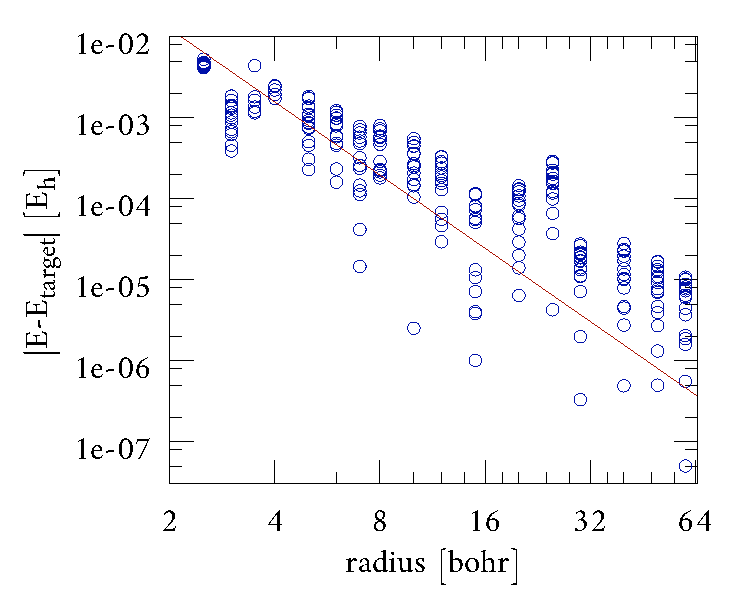
\includegraphics[width=\textwidth]{Figures/BC/BoxsInfEL}
\caption{a)Double-logarithmic plot of the error in energy for different radii of the finite element region.
b)-d) partial wave contribution \eq{eq:PartWaveCoeff} of the $15$ eigenenergies with smallest error;
the box-sizes are: b) $r_\text{max}=4\,$bohr; c) $r_\text{max}=8\,$bohr; d) $r_\text{max}=20\,$bohr and $N=20$ sheres are used in all cases.}
\label{fig:InfBoxs}
\end{figure}
On the other side, the angular momenta of the solutions are in general larger than those occurring with Dirichlet BC for the same box-size.
Moreover, the partial wave contributions (see \eq{eq:PartWaveCoeff}) shown in panels b) -- d) indicate that the angular momenta are much stronger mixed than in the case of Dirichlet BC which.
As discussed above, this is a direct consequence of the higher density of eigenenergies in this scheme.
The white space in the graphs c) and d) corresponds to contributions of angular momenta larger $l>7$ which are not computed here.
Most of the solutions obtained with box-sizes with $r_\text{max}>20\,$bohr, the contributions of angular momenta lower than $l=8$ vanish.
However, the appearance of solutions with significant contibutions of $l=2$ ($d$-wave) in figure \ref{fig:InfBoxs} d) shows that the growing angular momentum with increasing box-size is a general trend but does not hold strictly.

\subsubsection{Density of Spheres}
\label{sec:BenchSphere}
%Increasing the number of spheres has a considerable influence on the energies of FEFs but also changes the angular momenta of the solutions.
The influence of the number of spheres $N$ for a given box is another important parameter whose convergence-properties are important to understand.
A fundamental lower boundary for this is due to the wavelength of the function to be resembled.
However, a quantitative estimation of the convergence with respect to this number is not easy to make in general and depends on many further properties.

Numerical tests on this dependence for a given setup ($r_\text{max}=10\,$bohr and $E_\text{target}=0.5664\,$Hartree) are presented in Figure \ref{fig:InfNum}.
Similar to the behaviour found for Dirichlet BCs earlier in this work, a larger number of spheres leads to larger angular momenta as the comparison of the partial wave contributions in Figure \ref{fig:InfNum} for different numbers of spheres shows.

\begin{figure}[h]
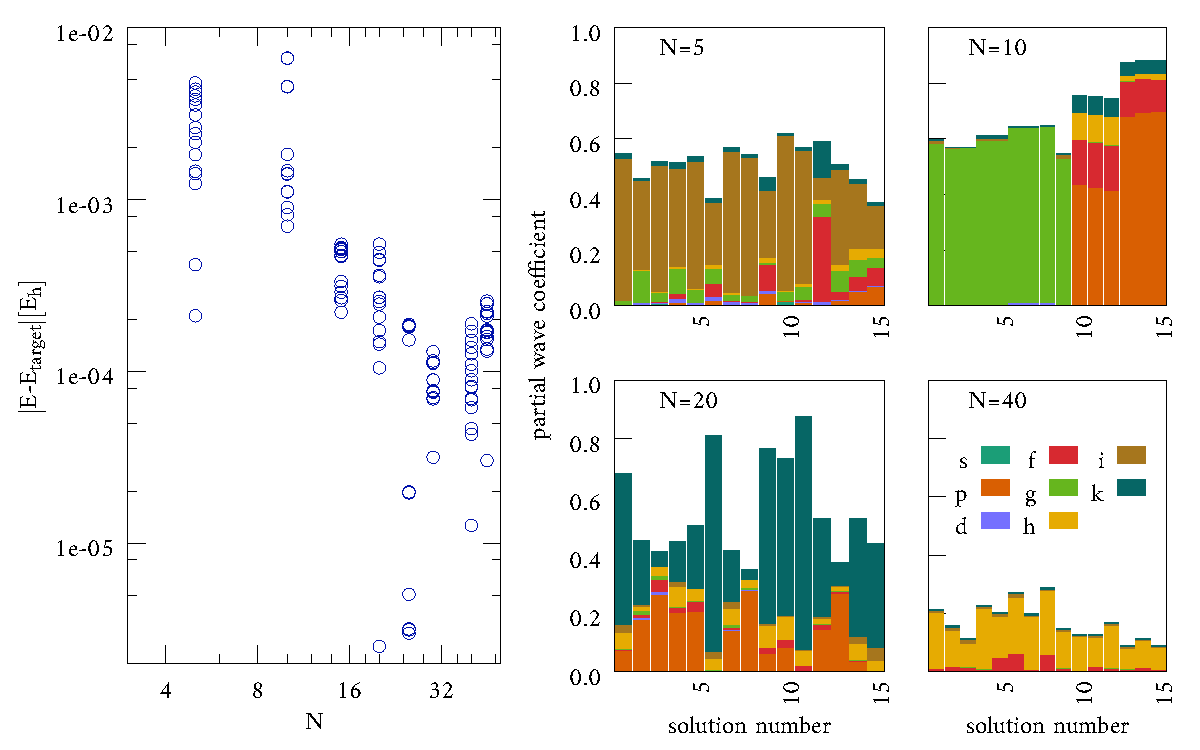
\includegraphics[width=\textwidth]{Figures/BC/NumInfEL}
\caption{The energy and partial wave contributions (\ref{eq:PartWaveCoeff}) for different number of spheres $N$ using infinite elements. The radius is $r_\text{max}=10\,$bohr, respectively.}
\label{fig:InfNum}
\end{figure}
Moreover, the error in energy shown in panel a) of Figure \ref{fig:InfNum} indicates that the shown configurations are far from saturation.
However, since high angular momenta are not desireable, a smaller number of spheres is better suited even though it is not converged.
Thus, the requirements of a low error in energy and high accuracy of the wave function are contrary to the need to have low angular momenta which are needed to obtain reasonable transition dipole moments.

In addition to this, the properties of the solutions presented in Figure \ref{fig:InfNum} change in an unsystematic way when the number of spheres $N$ increased.
As an example for this unsystematic behaviour, the energies of the FEFs obtained with $N=10$ spheres show a much largererror in energy than the solutions obtained with different setup.
The large error, in turn, is also reflected in a weak mixing of angular momenta as the comparison of panel c) with b), d) and f) shows.
%Not only the unsystematic behaviour, the strong dependence of the angular momentum on the number of spheres as such is surprising since, in principle, the radial and angular nodes should be represented with a similar quality.

\subsubsection{Radial Order}
Using the infinite element scheme, a set of additional basis functions is added to the finite element representation having form
\begin{equation} \label{eq:infAnsatzRep}
\Psi(r) = \left(\frac{a_1}{r} +\frac{a_2}{r^2} + \hdots \frac{a_{o}}{r^o} \right) e^{ikr}
\end{equation}
which corresponds to a truncated multipole expansion of order $o$.
As mentioned in section \ref{ch:InfEl}, the term with $o=1$ corresponds to the radial behaviour of an $s$-wave whereas higher radial orders describe the asymptotic behaviour of waves with respectively larger angular momentum.
\begin{figure}[h]
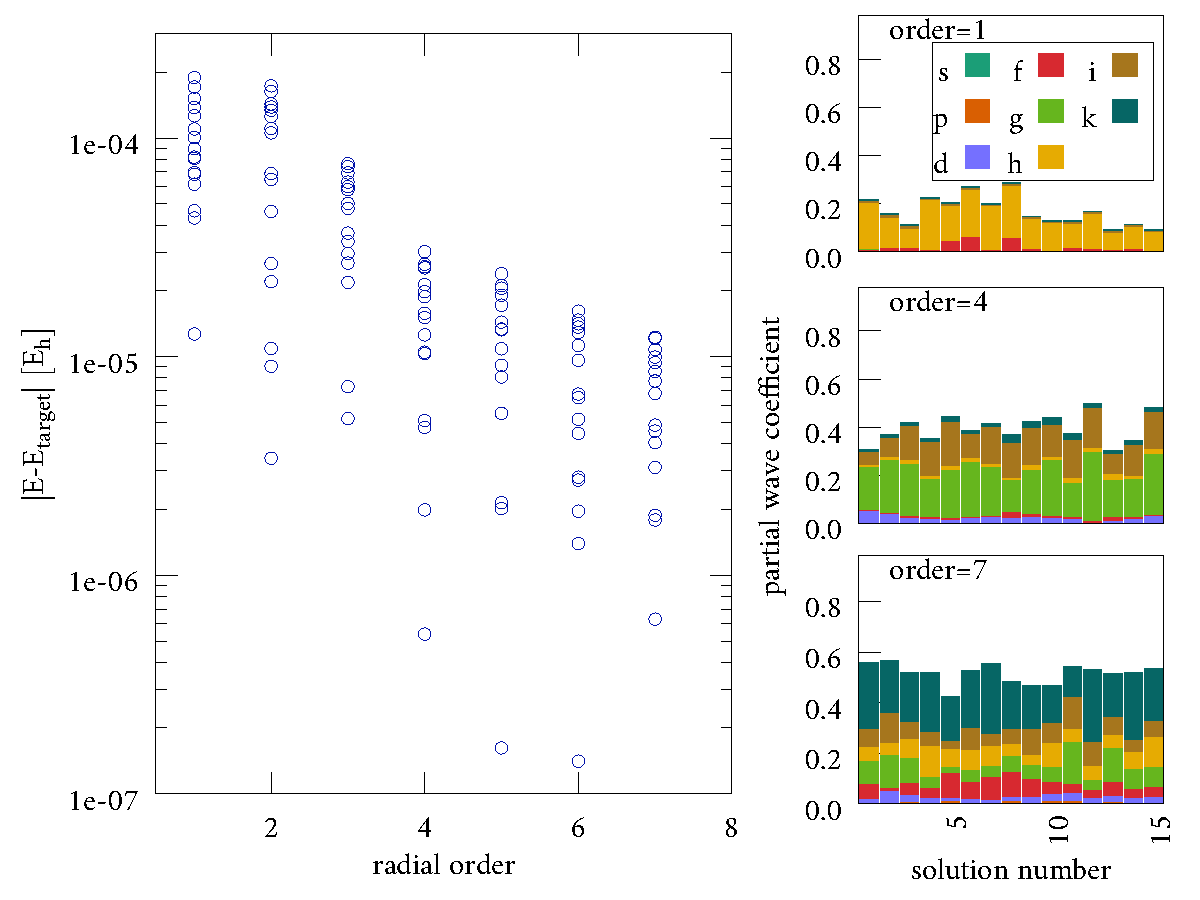
\includegraphics[width=\textwidth]{Figures/BC/OrdInfEL}
\caption{The error in energy for $15$ solutions obtained with a box with radius $r_\text{max}=10\,$bohr and $N=40$ spheres using different orders of the multipole expansion, see eq. (\ref{eq:InfansatzRep}).}
\label{fig:InfOrd}
\end{figure}

Having this in mind, the intuitive solution to the problems with large angular momenta and strong mixing of different contributions might be no restrict it by setting the maximum order $o$ to a respectively low value.
However, the results presented Figure \ref{fig:InfOrd} for different orders $o$ show a more intricate dependence.
The decreasing error in energy can be understood easily since a large amount of additional degrees of freedoms is added to the system.
However, a closer look at the character of the obtained solutions reveals that the angular momentum tends to decrease with larger orders in the multipole expansion \eq{eq:infAnsatzRep}.
The projection of the solutions onto spherical waves presented in Figure \ref{fig:InfOrd} shows that the computed FEFs have a partial wave contribution of about $0.2$ summed over all angular momenta up to 7 when only the first-order terms are taken into account.
However, the FEF with more degrees of freedom show by far larger contributions for the studied angular momenta.

\subsection{Conclusion on Boundary Conditions}
The study of different parameters has revealed several properties of the finite element setup.
An important conclusion of these tests is that a higher density of eigenenergies, which is considered as an indication for a more exact representation of the wave function, in general leads to the appearance of larger angular momenta and to strong coupling of different angular momentum contributions.
This dependence can be easily understood for the size of the computational domain $r_\text{max}$, since wave functions with larger angular momentum have a larger radial extend, but is not that straight forward in the case of number of spheres $N$.

Moreover, it was found that a high density of states usually leads to a stronger mixing of different angular momenta which seems to be a characteristic of this computational scheme.
However, the studies presented here show that a systematic setup of reasonable parameters is non-trivial and needs to  represent a compromise between a dense spectrum and reasonable radial dependence of the wave function on the one side, and low angular momenta as well as well-behaved solution on the other side.

\section{Energy Dependence of the Cross Sections}
\label{sec:cs}
The relative heights of different features in PESs are dependent on the energy of the incoming photons.
This dependence is small if the kinetic energy of the outgoing electron is high, but for low kinetic energies, \textit{i.e.} below $\approx 10\,$eV, the reproduction of the correct energy-dependence is important for a theoretical method to be able to predict the intensities in the PESs reliably.
In the DO formalism, this dependency is accounted for.
In general, the oscillations in the FEF become faster with increasing kinetic energy and thus, the overlap with thed DO, which usually has only few nodes, decreases.
In the limit of very fast oscillations the cross section becomes almost independent of kinetic energy, making the basis for the so-called sudden approximation \cite{saAberg}.
The main influence of this integral is the fact that the oscillations in the FEF become faster with increasing kinetic energy and thus, the overlap with the DO, which usually has only few nodes, decreases.
The slope of the decay with increasing photon energy thus contains information on the spatial extent of the DO.
For a broad and unstructured DO, the oscillations cancel most contributions out, whereas for a strongly localised DO is less sensitive to the wavelength.
%Moreover, a more complicated dependence of the intensity of a peak on kinetic energy including maxima indicates 
Thus, the dependence of the intensity of a peak on the photon energy contains information on the nature of the transition and is studied in a number of experimental and theoretical works for atomic systems as well as small molecules \cite{do_modCoul,LiNaRef1,LiCS,stieltje}.
In this work, the cross section of the valence transition of the lithium atom and the CO$_2$ molecule are studied.

In Figure \ref{fig:Li-CS}, the experimental intensity of the valence ionisation transition of lithium (binding energy of $E_b=0.2067\,$E$_\text{h}$) is shown as a function of the photon energy.
Since the kinetic energy (and thus the wavelength) of the particle spans over a very broad range, the computational setup for the FEF needs to be adapted to the particular kinetic energy of interest and should comprise some oscillations of the FEF in the discrete region.
The studies in section \ref{ch:BCbench} showed that the box-size is very critical to the properties of the solution.
It may not be too small to ensure a reasonable error in energy, but should not be too large to have considerable contributions of solutions with low angular momenta that is crucial for the computation of intensities due to the reasons discussed in section \ref{ch:BCbench}.
\begin{figure}
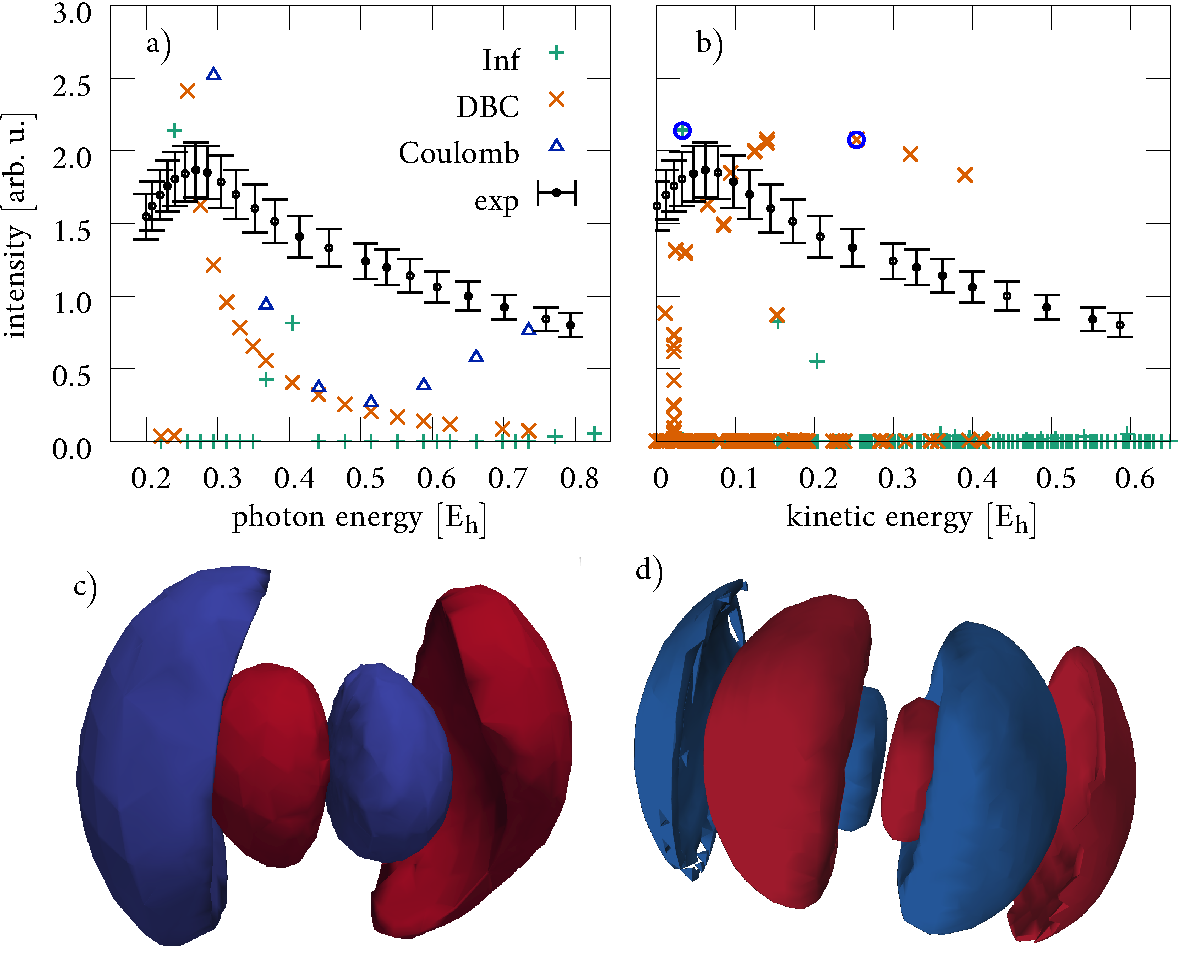
\includegraphics[width=\textwidth]{Figures/Lithium/CrossSect2}
\caption{a) The photoelectron cross section of the lithium atom as a function of the photon energy obtained by the FEM (Dirichlet BCs (DBC) and infinite elements (Inf)) and the Coulomb wave expansion (Coulomb), compared to experiment \cite{LiCS}.
The intensity is computed as sum over the intensities of $80$ FEFs;
b) The intensities corresponding to individual FEFs are shown.
c) and d) contour plots of the FEFs with the largest intensity contributions with Dirichlet BC (c) and with infinite elements (d), respectively.
Their corresponding peaks are marked in panel b). }
\label{fig:Li-CS}
\end{figure}
To account for this, the box-size was choosen to be $0.8\lambda$ in case of Dirichlet BC and $0.5\lambda$ for infinite elments, where $\lambda=\nicefrac{2\pi}{k}$ is the asymptotic wavelength (\textit{i.e.} reached outside the influence of the Coulomb potential) of the respective target energy.
The box-size smaller than $\lambda$ in case of Dirichlet BCs is too small for a reasonable error in energy but show, since the wavelength is considerably smaller in the presence of a Coulomb potential, still some radial nodes.
For all setups, $N=18$ spheres and the radial mapping scheme \textit{tm}, \eq{eq:tm_map}, with the parameters $q=2.5$ and $s=1.2$ was used, respectively.
For the infinite elements the radial polynomial is truncated after the first order to suppress higher angular momenta.

The intensities obtained with the finite element scheme are presented in two different ways in Figure \ref{fig:Li-CS}.
In the left panel, the $80$ energetically closest intensities are summed up whereas in the right panel the individual intensities are shown.
The theoretical results are scaled to be in good agreement with the experimental data.
For the results obtained with the Dirichlet BCs, the summed intensities (left panel of Figure \ref{fig:Li-CS}) show a systematic but qualitatively wrong behaviour which can be explained by the box which is considerably too small to ensure the correct shape of the wave-function.
However, the intensities of the single transitions (right panel of Figure \ref{fig:Li-CS}) have a different progression.
%Since their energetic position corresponds to their actual kinetic energy, it can be seen that the solutions obtained are in general energetically too low so that no transitions above $0.6\,$E$_\text{h}$ occur.
The qualitative difference between these schemes can be explained by the fact that in the right pannel at lower kinetic energies many transitions contribute with a considerable intensity whereas at higher kintetic energies only few solutions contribute.
Moreover, the transitions can be strongly reordered between the graphs since deviations between the target energy and eigenenergy of up to $0.11\,$Hartree occur.

The results obtained with infinite elements show a less systematic behaviour: Among the hundreds of solutions computed, only three contribute significantly to the cross section.
The scaling factor of the transitions shown in the right panel of Figure \ref{fig:Li-CS} are $0.7$ for the soltions obtained with the Dirichlet BC and $0.4$ for those computed with infinite elements, thus their relative scale is in the same order of magnitude.
These results show that, even for a small computational domain as it is used here, only a poor agreement with the experiment is achievable.
In case of Dirichlet BCs, the bad agreement with the experimental data can be explained by the size of the box which restricts the solution to low angular momenta but introduces a large error in the shape of the wave function and thus influences the dipole matrix elements considerably.
A study with a more reasonable radius of $r_\text{max}=3.5\lambda$ was conducted as well and is shown in Figure \ref{subfig:LiCS}.
However, even though the eigenenergies are denser and the wave function are more flexible, only few transitions with considerable intensity were obtained.
Another important question concerns the normalisation of the wave function.

In the case of infinite elements, too few transitions contributing to the intensity are obtained for an analysis of their kinetic-energy dependence.
However, this shows that even for such a small box, the angular momentum is in general too high to give considerable contributions, at least for $s$-type DOs.

\textcolor{green}{
\begin{itemize}
   \item Explain, why a systematic setup over such a wide range of kinetic energies is not possible for the given scheme. This problem can be seen esp. for DBC comparing left and right of \ref{fig:Li-CS}.\\
    This should be already the main reason for the unsystematic results!?
\end{itemize}
}

\textcolor[rgb]{1,0.7,0}{
   The intensities obtained with the Coulomb wave function are, similar to the results obtained with the FEM and Dirichlet BC, in poor agreement with the experimental data.
   Since the ESP of lithium is very close to that of hydrogen, this is surprising.
   Moreover, the shape makes no sense at all.
}

\textcolor{blue}{
For the computation of the overlap integral, only the finite region is taken into account since outside of it the DO vanishes and thus the outer region would not lead to further contributions.
In this region usually, the wave function is normalised to one which is, especially in the case of Dirichlet boundary conditions, the usual normalisation.
However, if the intensities obtained with different box-sizes are to be compared, two wave functions that coincide in the central region but are computed on differently large regions would result in different intensities.
To account for this, here the wave functions are normalised to the volume, \textit{i.e.}
\begin{equation}
\int_V \left|\Psi_n (\vec{r})\right|^2d\vec{r}=\int d\vec{r}=V
\end{equation}
where $V$ is the volume of the finite element region.}

\textcolor{red}{
For the second testing-system, here first the PES as a whole should be discussed.
\begin{itemize}
   \item assign transitions
   \item The first IP is reproduced well, due to OTRSH-scheme used.
   \item The positions of the other bands are strentched
   \item A considerable part of the features not reproduced, since vibronic progression is not studied here;
   \item SA and DOS are similar (!?) integration changes heights -> improves agreement with experiment.
\end{itemize}
}

For the first two transitions, that correspond to degenerate DOs with $\pi$-character respectively, here also the cross section dependence on the photon energy is studied.
In Figure \ref{fig:CO2CS}, the energy-dependence of the first two transitions shown in Figure \textcolor{red}{that showing the PES} is shown as obtained with various theoretical methods.
\begin{figure}
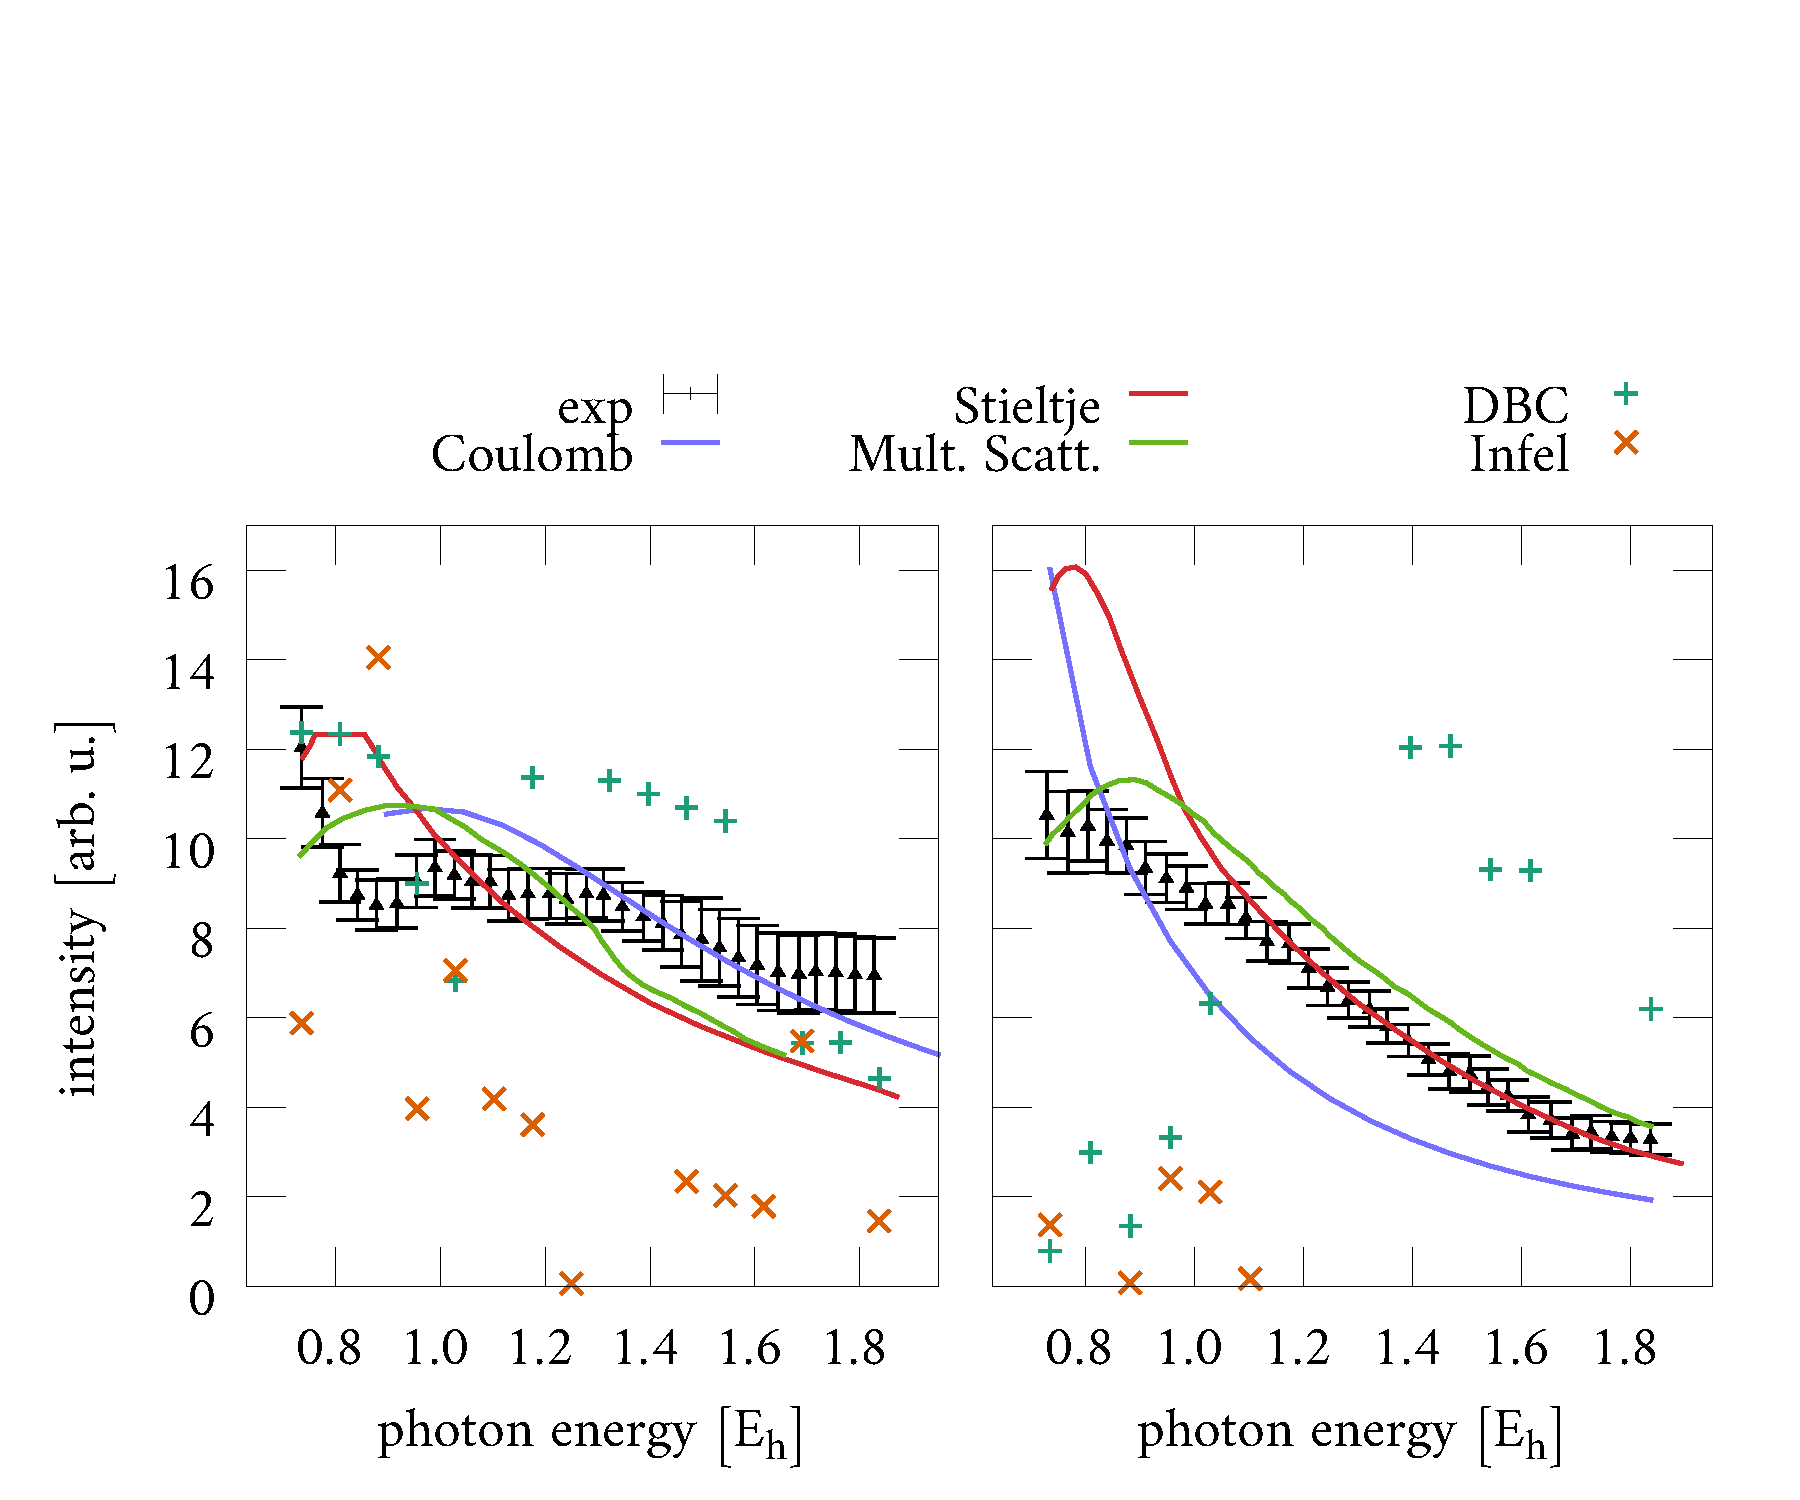
\includegraphics[width=\textwidth]{Figures/CO2/CrossSect}
\caption{\textcolor{red}{Add labels!} The intensity of the two energetically highest transitions of CO$_2$ as a function of photon energy.}
\label{fig:CO2CS}
\end{figure}
Comparing the results obtained with the multiple scattering method \textcolor{green}{citation} and the Stieltjes imaging approach \cite{stieltje}, a reasonable agreement is achieved.
Both approaches reproduce the main behaviour of the function.
However, for small kinetic energies, both methods do not reproduce the experimental data that well.
The larger problems in case of the $\pi_g$-transition (Figure \ref{fig:CO2CS}) can be explained by the higher binding energy of $...$ and thus lower kinetic energy compared to the $\pi_u$-transition whose cross section is shown in Figure \ref{fig:CO2CS}.

The respective results obtained with the Coulomb wave expansion show also good agreement in case of the $\pi_g$-transition.
In the case of the $\pi_g$-transition, the intensity is highly overestimated for lower photon energies but shows a similar dependence for photon energies larger than about $1.3\,$Hartree.
The good agreement of the results obtained with the approach using a Coulomb wave shows that this approach is more reliable than one might expect, even for highly non-spherical systems such as CO$_2$.
Similar results have been abtained also by Gozem \textit{et.al} who investigated the photoenergy dependence of various transitions of atomic and small molecular systems and showed that the charge $Z$ in the expression for Coulomb waves can be tuned such that an overall good agreemence is achieved \cite{do_modCoul}.

Studying the intensity of these two transitions with the finite element protocol developed here, shows, similar to the results of lithium shown in Figure \ref{fig:Li-CS}, a very unsystematic behaviour.
However, for both transitions studied here, at least a general trend can be extracted which is very similar for both BCs used.
In the Figure \ref{fig:COC2S} a) this trend is in good agreement with the experimental values.
However, the intensities computed for low photon energies in Figure \ref{fig:CO2CS} indicate, that the scheme in use is also not well-suited for the case of low kinetic energies.
It is important to note at this point that the results obtained here have in general a too unsystematic behaviour to draw reliable conclusions from these results.

Despite the problems of finding a setup for which the properties of the solutions can be governed in a reasonable way are addressed above already. \textcolor{blue}{<-reformulate!}
However, in addition to this, another general question arises when using multiple FEFs for determining the intensiy of a transition is that for convergence.
While it is clear that the use of one particular solution for the computation of intensities is in general not a valid scheme, the summation over multiple solutions is only reliable if it converges at a predictible number of states being used.
\begin{figure}
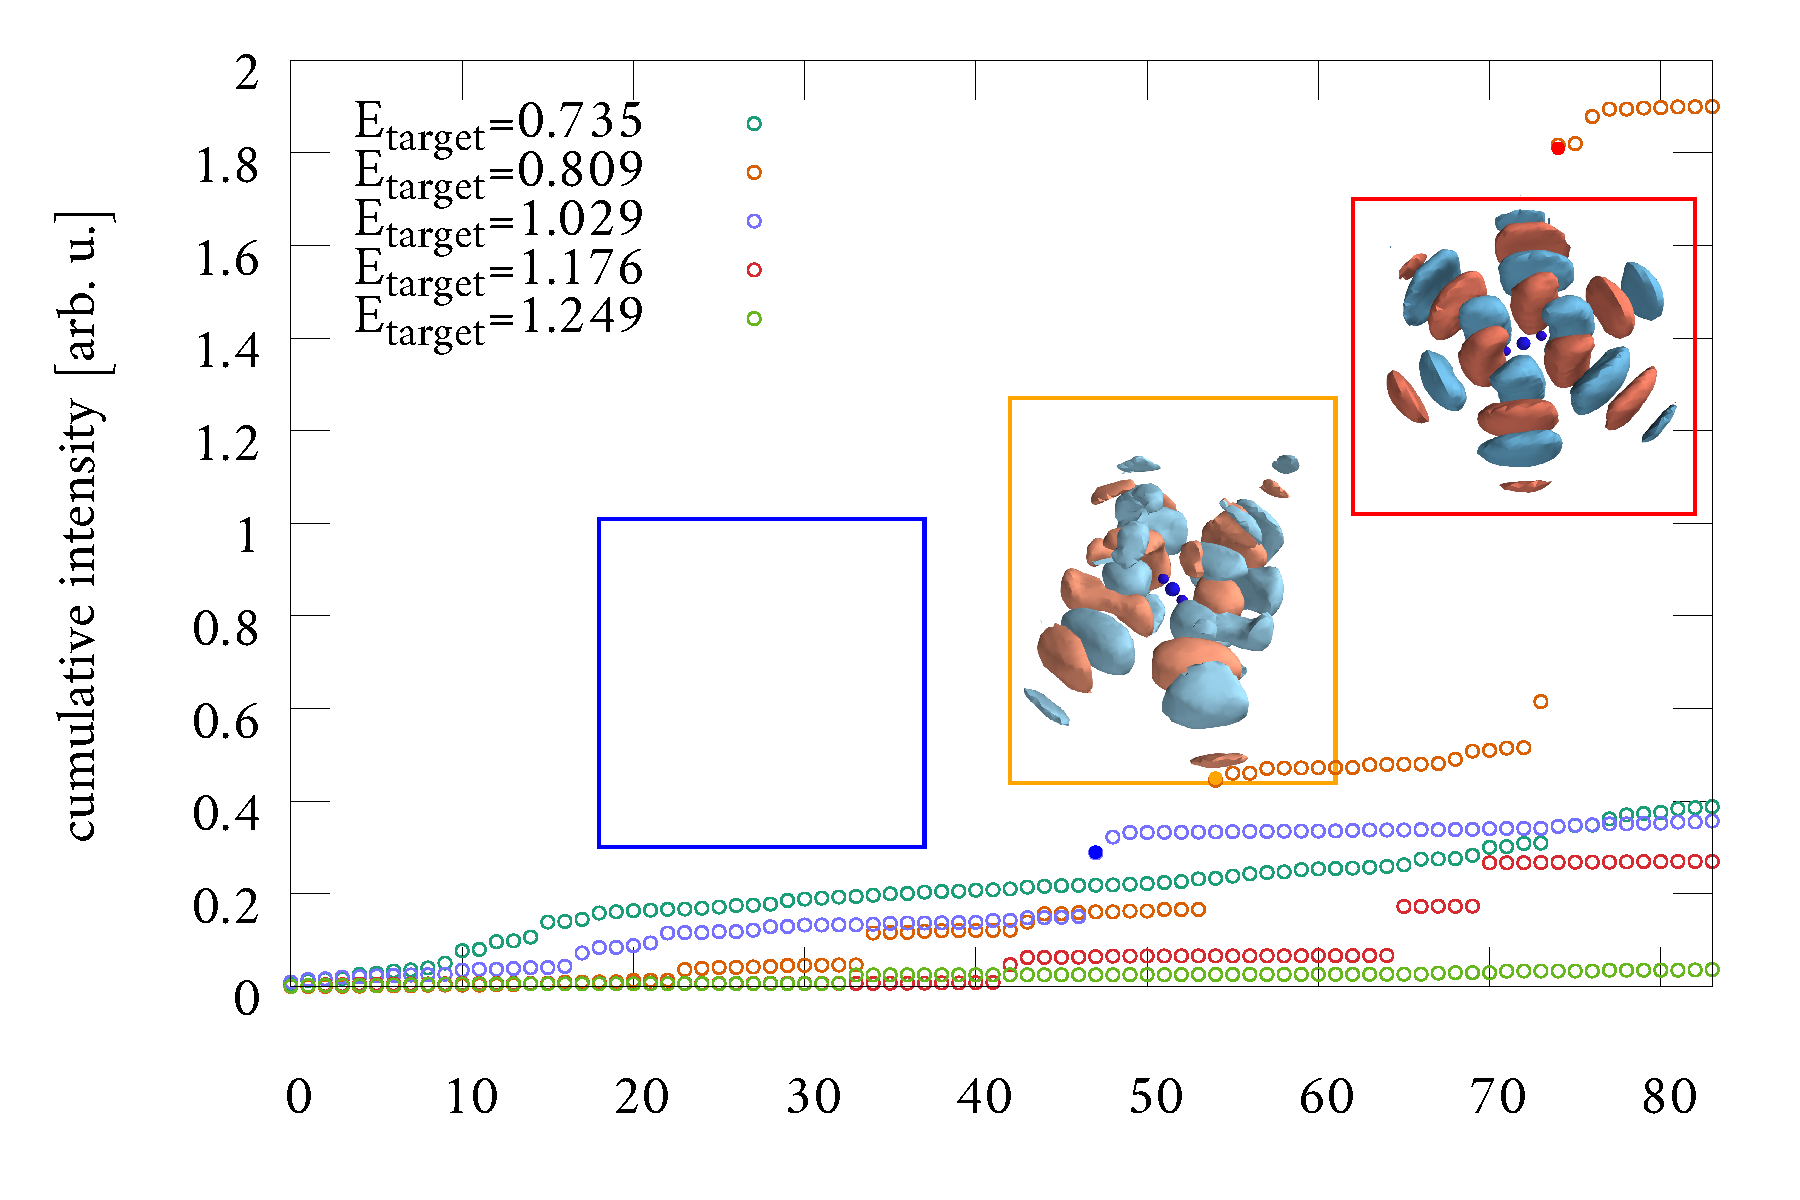
\includegraphics[width=\textwidth]{Figures/CO2/Cronverge}
\caption{Convergence of intensities for the $\pi_g$-transition of CO$_2$.}
\label{fig:cronverge}
\end{figure}
In Figure \ref{fig:croverge}, such a study is shown for the intensities obtained for one of the degenerate $\pi_g$-DOs at different photon energies.
Similar to the studies shown above, here also the radius of the computational domain is adapted to the wavelength.
The cross section here is summed over all states up to the given solution.
The FEF contributing most to the intensities of the studied configurations are shown in the graph to illustrate ????.
As the comparison of the development of the different solution shows, here no convergence is reached.
Instead, the continuum functions with considerable contributions to the transition strength are not systematically distributed.

With this there is no hope anymore. So lets make something different:

Figure \ref{fig:benzPES} shows the PES of benzene obtained with this setup using a grid of height (orthogonal to the molecular plane) of $8\,$\AA\, and a diameter of $12$\AA\, in both directions of the molecular plane with $380$ points in each direction.
\begin{wrapfigure}{L}{0.5\textwidth}
%\begin{figure}
   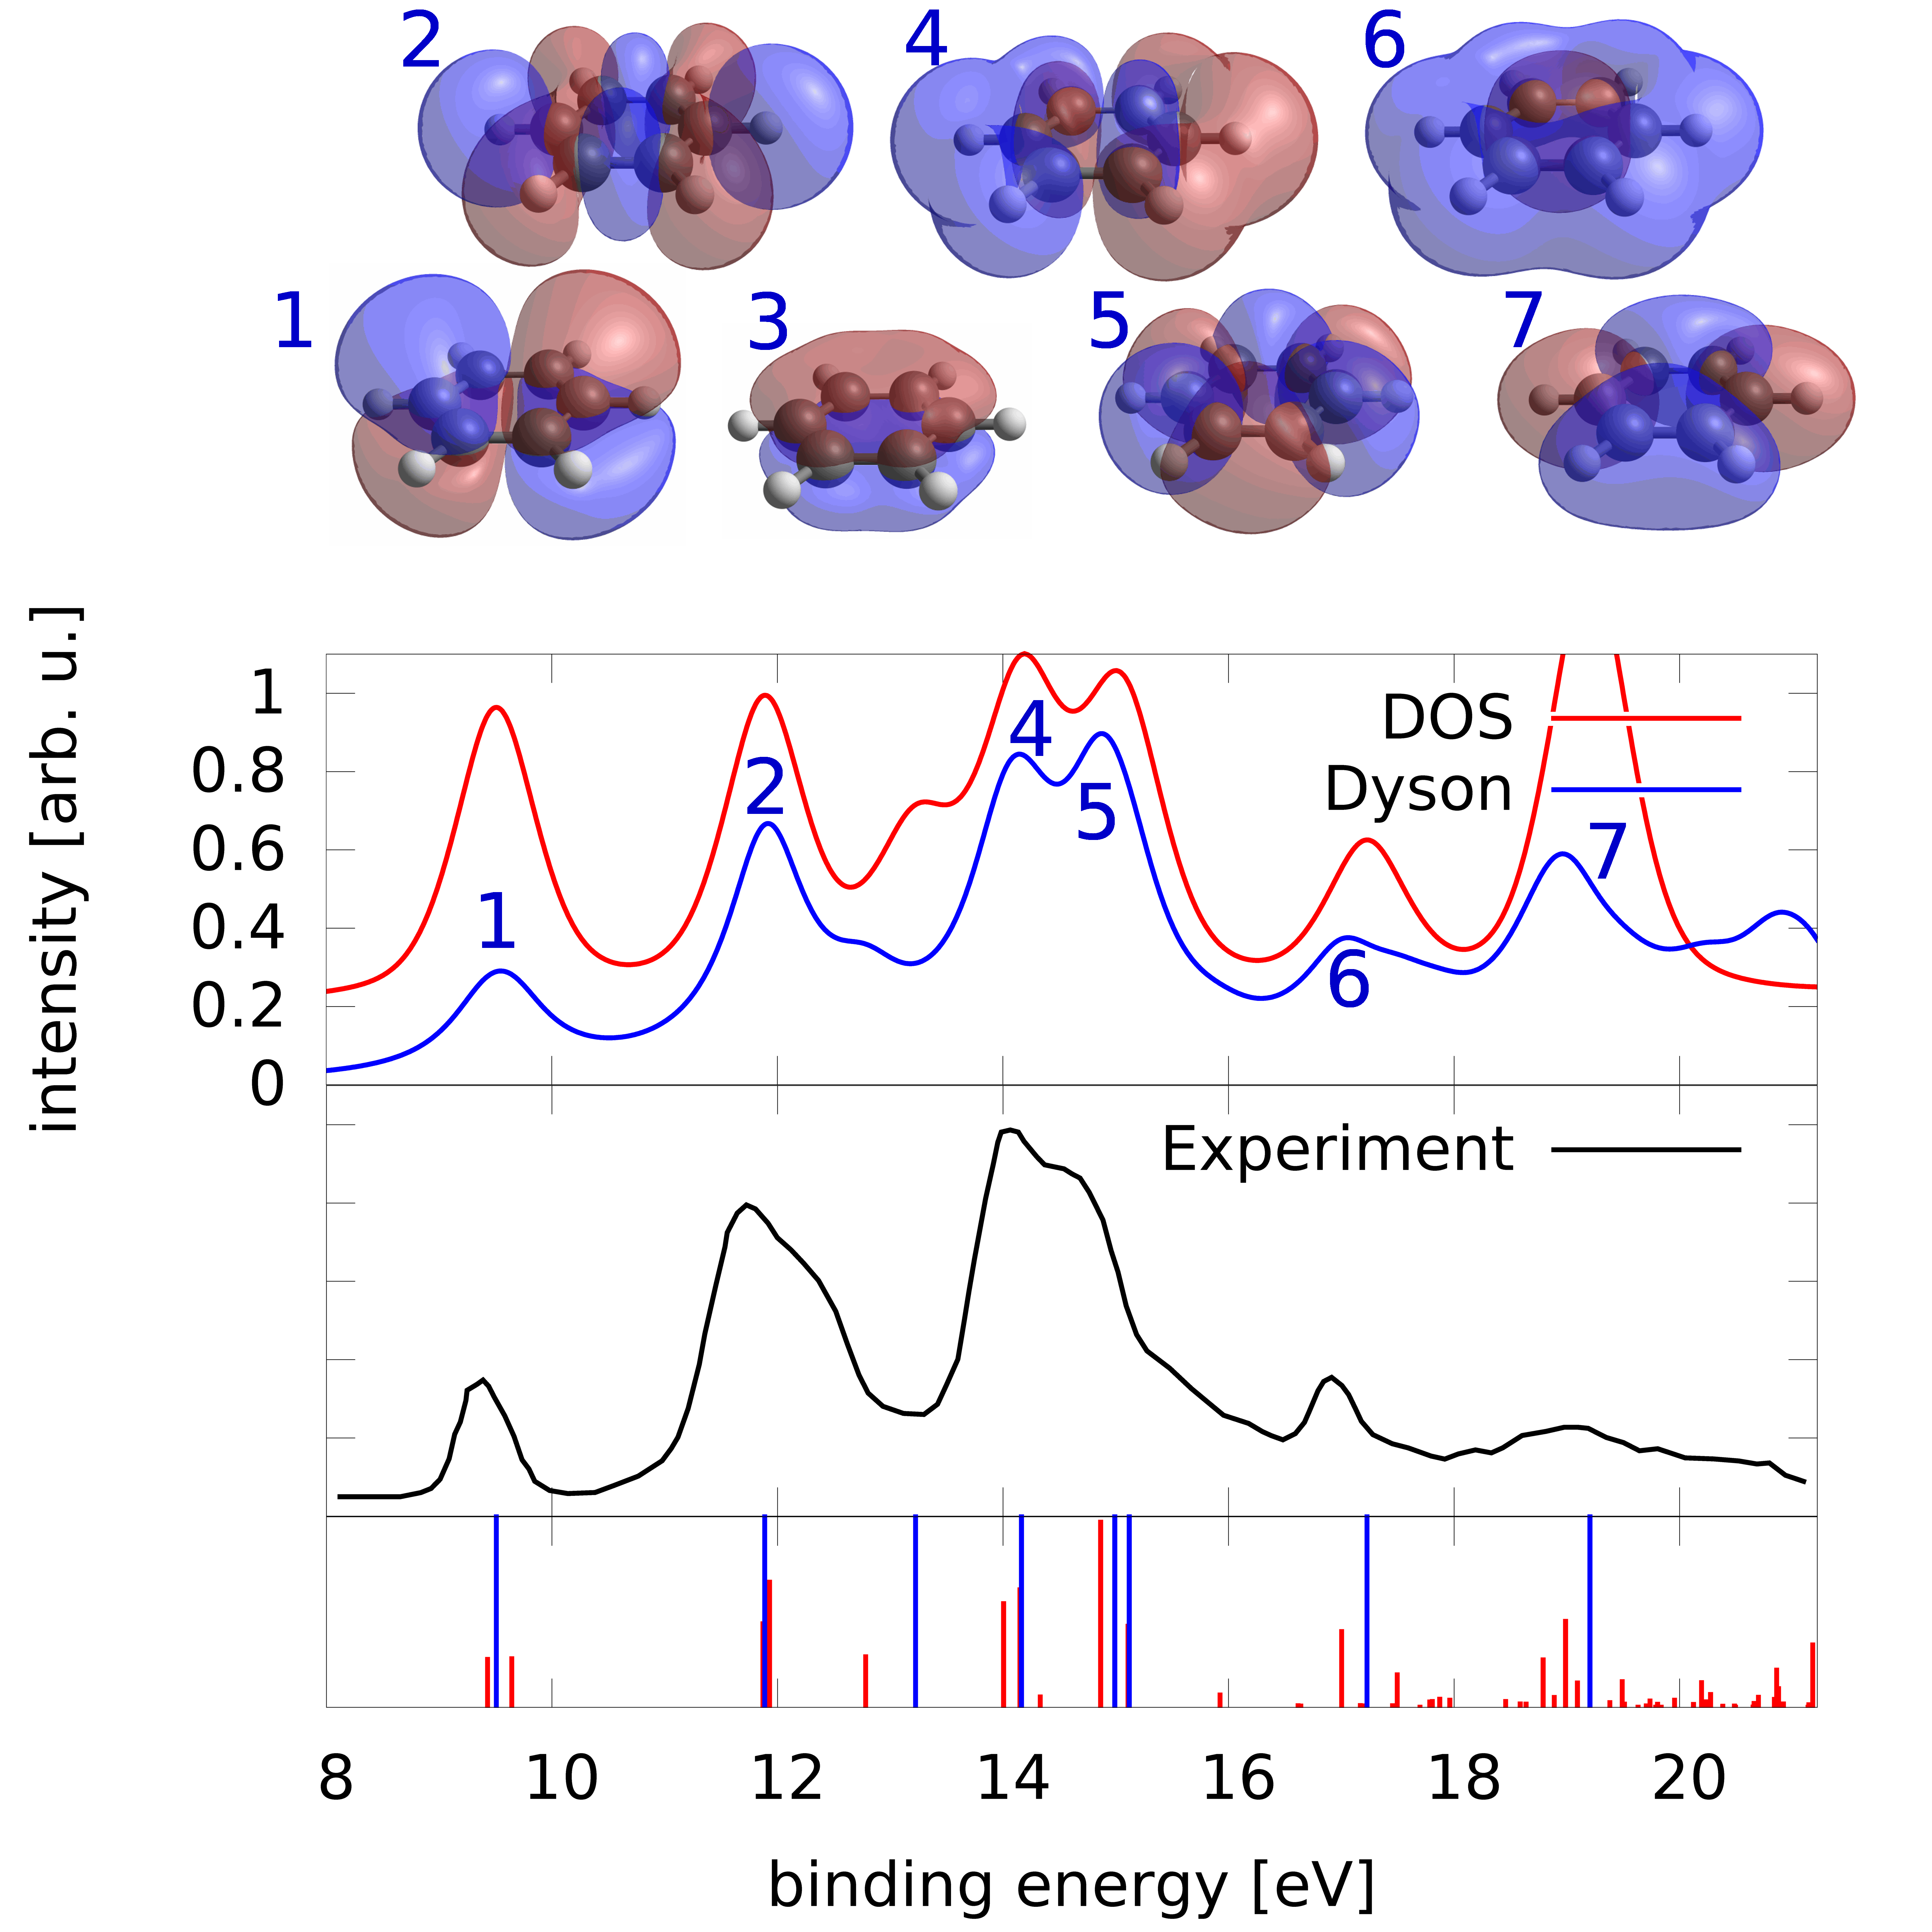
\includegraphics[width=0.5\textwidth]{Figures/Benzene/Benzene}
   \caption{Photoelectron spectra of benzene at different levels of theory.
   In the upper panel the spectra obtained with the Dyson orbital formalism (Dyson) and using the Koopmans' approach (DOS) are compared, the experimental reference is shown in the lower panel \cite{BenzExp}.}
   \label{fig:benzPES}
%\end{figure}
\end{wrapfigure}
The expansion of Coulomb waves includes the terms up to an angular momentum of $l=10$.
The second spectrum shown in 
To indicate the consequences of the OTRSH procedure, in Figure \ref{fig:blypPES} the PES of benzene as predicted with the optimised functional and the B3LYP functional are shown.
For this system, the agreement is good, for other systems the differences are much larger as the example of S$_8$ in the supplement shows.
\begin{figure}
   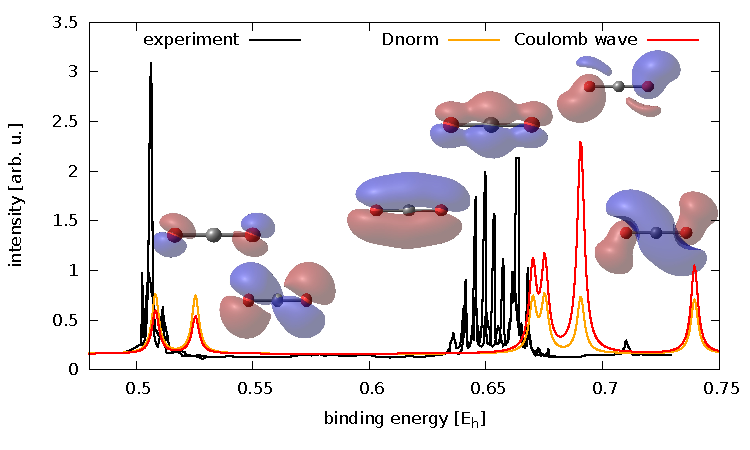
\includegraphics[width=0.8\textwidth]{Figures/CO2/CO2_spect}
   \caption{}
\end{figure}
\textcolor{red}{
OTRSH is known no be not very good for linear molecules --> is there some reason for this?
}
